\documentclass{book}
\usepackage[a4paper,top=2.5cm,bottom=2.5cm,left=2.5cm,right=2.5cm]{geometry}
\usepackage{makeidx}
\usepackage{natbib}
\usepackage{graphicx}
\usepackage{multicol}
\usepackage{float}
\usepackage{listings}
\usepackage{color}
\usepackage{ifthen}
\usepackage[table]{xcolor}
\usepackage{textcomp}
\usepackage{alltt}
\usepackage{ifpdf}
\ifpdf
\usepackage[pdftex,
            pagebackref=true,
            colorlinks=true,
            linkcolor=blue,
            unicode
           ]{hyperref}
\else
\usepackage[ps2pdf,
            pagebackref=true,
            colorlinks=true,
            linkcolor=blue,
            unicode
           ]{hyperref}
\usepackage{pspicture}
\fi
\usepackage[utf8]{inputenc}
\usepackage{mathptmx}
\usepackage[scaled=.90]{helvet}
\usepackage{courier}
\usepackage{sectsty}
\usepackage[titles]{tocloft}
\usepackage{doxygen}
\lstset{language=C++,inputencoding=utf8,basicstyle=\footnotesize,breaklines=true,breakatwhitespace=true,tabsize=8,numbers=left }
\makeindex
\setcounter{tocdepth}{3}
\renewcommand{\footrulewidth}{0.4pt}
\renewcommand{\familydefault}{\sfdefault}
\hfuzz=15pt
\setlength{\emergencystretch}{15pt}
\hbadness=750
\tolerance=750
\begin{document}
\hypersetup{pageanchor=false,citecolor=blue}
\begin{titlepage}
\vspace*{7cm}
\begin{center}
{\Large Mark I\-X }\\
\vspace*{1cm}
{\large Generated by Doxygen 1.8.1}\\
\vspace*{0.5cm}
{\small Thu May 31 2012 13:02:15}\\
\end{center}
\end{titlepage}
\clearemptydoublepage
\pagenumbering{roman}
\tableofcontents
\clearemptydoublepage
\pagenumbering{arabic}
\hypersetup{pageanchor=true,citecolor=blue}
\chapter{Logging C\-R\-I\-O Competition Page}
\label{index}\hypertarget{index}{}\begin{DoxyVerb}This is the Robot Code for the 2012 Season of Rebound Rumble
\end{DoxyVerb}


If you haven't already, please visit our \href{http://www.amhsrobotics.com}{\tt website}. 
\chapter{Class Index}
\section{Class Hierarchy}
This inheritance list is sorted roughly, but not completely, alphabetically\-:\begin{DoxyCompactList}
\item \contentsline{section}{Atom}{\pageref{class_atom}}{}
\begin{DoxyCompactList}
\item \contentsline{section}{Line\-Atom}{\pageref{class_line_atom}}{}
\item \contentsline{section}{Pause\-Atom}{\pageref{class_pause_atom}}{}
\item \contentsline{section}{Shoot\-Atom}{\pageref{class_shoot_atom}}{}
\item \contentsline{section}{Turn\-Atom}{\pageref{class_turn_atom}}{}
\item \contentsline{section}{Wrist\-Atom}{\pageref{class_wrist_atom}}{}
\end{DoxyCompactList}
\item \contentsline{section}{Auto\-Target}{\pageref{class_auto_target}}{}
\item \contentsline{section}{Auto\-Target\-Test}{\pageref{class_auto_target_test}}{}
\item \contentsline{section}{Drive\-Train}{\pageref{class_drive_train}}{}
\item \contentsline{section}{log\-File}{\pageref{structlog_file}}{}
\item \contentsline{section}{Mark\-I\-X}{\pageref{class_mark_i_x}}{}
\item \contentsline{section}{Molecule}{\pageref{class_molecule}}{}
\item \contentsline{section}{Pneumatic\-Controller}{\pageref{class_pneumatic_controller}}{}
\item \contentsline{section}{Pneumatics}{\pageref{class_pneumatics}}{}
\item \contentsline{section}{Pneumatic\-Test}{\pageref{class_pneumatic_test}}{}
\item \contentsline{section}{Robot\-Demo}{\pageref{class_robot_demo}}{}
\item \contentsline{section}{Task\-Test}{\pageref{class_task_test}}{}
\item \contentsline{section}{Testing}{\pageref{class_testing}}{}
\item \contentsline{section}{T\-K\-O\-Camera}{\pageref{class_t_k_o_camera}}{}
\item \contentsline{section}{T\-K\-O\-Conveyor}{\pageref{class_t_k_o_conveyor}}{}
\item \contentsline{section}{T\-K\-O\-Gyro}{\pageref{class_t_k_o_gyro}}{}
\item \contentsline{section}{T\-K\-O\-Intake}{\pageref{class_t_k_o_intake}}{}
\item \contentsline{section}{T\-K\-O\-Jaguar\-Controller}{\pageref{class_t_k_o_jaguar_controller}}{}
\item \contentsline{section}{T\-K\-O\-Joystick}{\pageref{class_t_k_o_joystick}}{}
\item \contentsline{section}{T\-K\-O\-Logging}{\pageref{class_t_k_o_logging}}{}
\item \contentsline{section}{T\-K\-O\-Relay}{\pageref{class_t_k_o_relay}}{}
\item \contentsline{section}{T\-K\-O\-Shooter}{\pageref{class_t_k_o_shooter}}{}
\item \contentsline{section}{T\-K\-O\-Turret}{\pageref{class_t_k_o_turret}}{}
\end{DoxyCompactList}

\chapter{Class Index}
\section{Class List}
Here are the classes, structs, unions and interfaces with brief descriptions\-:\begin{DoxyCompactList}
\item\contentsline{section}{\hyperlink{class_atom}{Atom} }{\pageref{class_atom}}{}
\item\contentsline{section}{\hyperlink{class_auto_target}{Auto\-Target} }{\pageref{class_auto_target}}{}
\item\contentsline{section}{\hyperlink{class_auto_target_test}{Auto\-Target\-Test} }{\pageref{class_auto_target_test}}{}
\item\contentsline{section}{\hyperlink{class_drive_train}{Drive\-Train} }{\pageref{class_drive_train}}{}
\item\contentsline{section}{\hyperlink{class_line_atom}{Line\-Atom} }{\pageref{class_line_atom}}{}
\item\contentsline{section}{\hyperlink{structlog_file}{log\-File} }{\pageref{structlog_file}}{}
\item\contentsline{section}{\hyperlink{class_mark_i_x}{Mark\-I\-X} }{\pageref{class_mark_i_x}}{}
\item\contentsline{section}{\hyperlink{class_molecule}{Molecule} }{\pageref{class_molecule}}{}
\item\contentsline{section}{\hyperlink{class_pause_atom}{Pause\-Atom} }{\pageref{class_pause_atom}}{}
\item\contentsline{section}{\hyperlink{class_pneumatic_controller}{Pneumatic\-Controller} }{\pageref{class_pneumatic_controller}}{}
\item\contentsline{section}{\hyperlink{class_pneumatics}{Pneumatics} }{\pageref{class_pneumatics}}{}
\item\contentsline{section}{\hyperlink{class_pneumatic_test}{Pneumatic\-Test} }{\pageref{class_pneumatic_test}}{}
\item\contentsline{section}{\hyperlink{class_robot_demo}{Robot\-Demo} }{\pageref{class_robot_demo}}{}
\item\contentsline{section}{\hyperlink{class_shoot_atom}{Shoot\-Atom} }{\pageref{class_shoot_atom}}{}
\item\contentsline{section}{\hyperlink{class_task_test}{Task\-Test} }{\pageref{class_task_test}}{}
\item\contentsline{section}{\hyperlink{class_testing}{Testing} }{\pageref{class_testing}}{}
\item\contentsline{section}{\hyperlink{class_t_k_o_camera}{T\-K\-O\-Camera} }{\pageref{class_t_k_o_camera}}{}
\item\contentsline{section}{\hyperlink{class_t_k_o_conveyor}{T\-K\-O\-Conveyor} }{\pageref{class_t_k_o_conveyor}}{}
\item\contentsline{section}{\hyperlink{class_t_k_o_gyro}{T\-K\-O\-Gyro} }{\pageref{class_t_k_o_gyro}}{}
\item\contentsline{section}{\hyperlink{class_t_k_o_intake}{T\-K\-O\-Intake} }{\pageref{class_t_k_o_intake}}{}
\item\contentsline{section}{\hyperlink{class_t_k_o_jaguar_controller}{T\-K\-O\-Jaguar\-Controller} }{\pageref{class_t_k_o_jaguar_controller}}{}
\item\contentsline{section}{\hyperlink{class_t_k_o_joystick}{T\-K\-O\-Joystick} }{\pageref{class_t_k_o_joystick}}{}
\item\contentsline{section}{\hyperlink{class_t_k_o_logging}{T\-K\-O\-Logging} }{\pageref{class_t_k_o_logging}}{}
\item\contentsline{section}{\hyperlink{class_t_k_o_relay}{T\-K\-O\-Relay} }{\pageref{class_t_k_o_relay}}{}
\item\contentsline{section}{\hyperlink{class_t_k_o_shooter}{T\-K\-O\-Shooter} }{\pageref{class_t_k_o_shooter}}{}
\item\contentsline{section}{\hyperlink{class_t_k_o_turret}{T\-K\-O\-Turret} }{\pageref{class_t_k_o_turret}}{}
\item\contentsline{section}{\hyperlink{class_turn_atom}{Turn\-Atom} }{\pageref{class_turn_atom}}{}
\item\contentsline{section}{\hyperlink{class_wrist_atom}{Wrist\-Atom} }{\pageref{class_wrist_atom}}{}
\end{DoxyCompactList}

\chapter{Class Documentation}
\hypertarget{class_atom}{\section{Atom Class Reference}
\label{class_atom}\index{Atom@{Atom}}
}
Inheritance diagram for Atom\-:\begin{figure}[H]
\begin{center}
\leavevmode
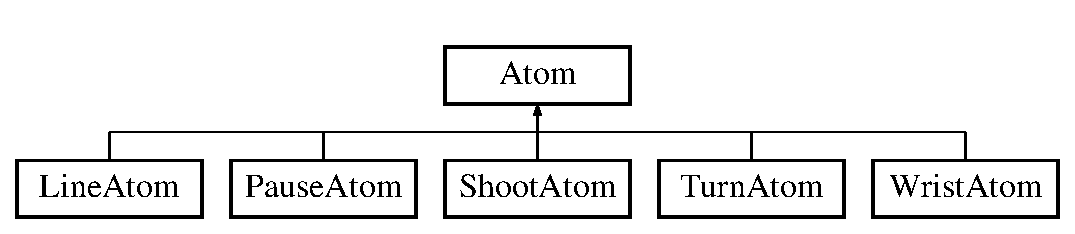
\includegraphics[height=2.000000cm]{class_atom}
\end{center}
\end{figure}
\subsection*{Public Member Functions}
\begin{DoxyCompactItemize}
\item 
\hypertarget{class_atom_af41beeaa245ff5f6e861ee4d76727984}{{\bfseries Atom} (C\-A\-N\-Jaguar $\ast$front\-Left, C\-A\-N\-Jaguar $\ast$rear\-Left, C\-A\-N\-Jaguar $\ast$front\-Right, C\-A\-N\-Jaguar $\ast$rear\-Right)}\label{class_atom_af41beeaa245ff5f6e861ee4d76727984}

\item 
\hypertarget{class_atom_a608318a9ac265ad2a30a62f501ff49d0}{virtual void {\bfseries Execute} ()=0}\label{class_atom_a608318a9ac265ad2a30a62f501ff49d0}

\item 
\hypertarget{class_atom_aad04a35d097df751c0e7196d29dc0d1d}{virtual bool {\bfseries Done} ()}\label{class_atom_aad04a35d097df751c0e7196d29dc0d1d}

\end{DoxyCompactItemize}
\subsection*{Protected Attributes}
\begin{DoxyCompactItemize}
\item 
\hypertarget{class_atom_a8b9a3812a495585b246b569d976722ee}{C\-A\-N\-Jaguar $\ast$ {\bfseries \-\_\-front\-Left}}\label{class_atom_a8b9a3812a495585b246b569d976722ee}

\item 
\hypertarget{class_atom_a1dbf54b07a056e8a7e0a9e5ce9013e03}{C\-A\-N\-Jaguar $\ast$ {\bfseries \-\_\-rear\-Left}}\label{class_atom_a1dbf54b07a056e8a7e0a9e5ce9013e03}

\item 
\hypertarget{class_atom_aa8930a2b7b54aa581274033899f7761d}{C\-A\-N\-Jaguar $\ast$ {\bfseries \-\_\-front\-Right}}\label{class_atom_aa8930a2b7b54aa581274033899f7761d}

\item 
\hypertarget{class_atom_a69d083ed75359c1eab8b3054a6fab0e2}{C\-A\-N\-Jaguar $\ast$ {\bfseries \-\_\-rear\-Right}}\label{class_atom_a69d083ed75359c1eab8b3054a6fab0e2}

\item 
\hypertarget{class_atom_a4a17c1192d97b4d5a32e75d3e58f0f63}{bool {\bfseries \-\_\-done}}\label{class_atom_a4a17c1192d97b4d5a32e75d3e58f0f63}

\item 
\hypertarget{class_atom_aa2099b75919bcbe34e95cbb5f1837956}{bool {\bfseries \-\_\-started}}\label{class_atom_aa2099b75919bcbe34e95cbb5f1837956}

\end{DoxyCompactItemize}


The documentation for this class was generated from the following files\-:\begin{DoxyCompactItemize}
\item 
Varun\-\_\-\-Atoms/Atom.\-h\item 
Varun\-\_\-\-Atoms/Atom.\-cpp\end{DoxyCompactItemize}

\hypertarget{class_auto_target}{\section{Auto\-Target Class Reference}
\label{class_auto_target}\index{Auto\-Target@{Auto\-Target}}
}
\subsection*{Public Member Functions}
\begin{DoxyCompactItemize}
\item 
\hypertarget{class_auto_target_a99d14582c957613ce4b007cab6cb4ede}{void {\bfseries Set\-Status} (bool status)}\label{class_auto_target_a99d14582c957613ce4b007cab6cb4ede}

\item 
\hypertarget{class_auto_target_a923ff75bce82fef677272478e969b753}{bool {\bfseries Get\-Status} ()}\label{class_auto_target_a923ff75bce82fef677272478e969b753}

\item 
\hypertarget{class_auto_target_a87bad0bcf59c89acf6874535a3d8f2f1}{\hyperlink{class_t_k_o_camera}{T\-K\-O\-Camera} $\ast$ {\bfseries Get\-Camera} ()}\label{class_auto_target_a87bad0bcf59c89acf6874535a3d8f2f1}

\item 
\hypertarget{class_auto_target_a4f3677b29010b28441f39e8891ff8e53}{\hyperlink{class_t_k_o_turret}{T\-K\-O\-Turret} $\ast$ {\bfseries Get\-Turret} ()}\label{class_auto_target_a4f3677b29010b28441f39e8891ff8e53}

\end{DoxyCompactItemize}


The documentation for this class was generated from the following files\-:\begin{DoxyCompactItemize}
\item 
Tanay\-\_\-\-Auto\-Targetting/Auto\-Target.\-h\item 
Tanay\-\_\-\-Auto\-Targetting/Auto\-Target.\-cpp\end{DoxyCompactItemize}

\hypertarget{class_auto_target_test}{\section{Auto\-Target\-Test Class Reference}
\label{class_auto_target_test}\index{Auto\-Target\-Test@{Auto\-Target\-Test}}
}
\subsection*{Public Member Functions}
\begin{DoxyCompactItemize}
\item 
void \hyperlink{class_auto_target_test_a718386ba75b9472eb51a78a63c1eb8fd}{Autonomous} (void)
\item 
void \hyperlink{class_auto_target_test_a530cef7a8526676787341aebd9f60314}{Operator\-Control} (void)
\end{DoxyCompactItemize}


\subsection{Detailed Description}
This is a demo program showing the use of the Robot\-Base class. The Simple\-Robot class is the base of a robot application that will automatically call your Autonomous and Operator\-Control methods at the right time as controlled by the switches on the driver station or the field controls. 

\subsection{Member Function Documentation}
\hypertarget{class_auto_target_test_a718386ba75b9472eb51a78a63c1eb8fd}{\index{Auto\-Target\-Test@{Auto\-Target\-Test}!Autonomous@{Autonomous}}
\index{Autonomous@{Autonomous}!AutoTargetTest@{Auto\-Target\-Test}}
\subsubsection[{Autonomous}]{\setlength{\rightskip}{0pt plus 5cm}void Auto\-Target\-Test\-::\-Autonomous (
\begin{DoxyParamCaption}
\item[{void}]{}
\end{DoxyParamCaption}
)\hspace{0.3cm}{\ttfamily [inline]}}}\label{class_auto_target_test_a718386ba75b9472eb51a78a63c1eb8fd}
Drive left \& right motors for 2 seconds then stop \hypertarget{class_auto_target_test_a530cef7a8526676787341aebd9f60314}{\index{Auto\-Target\-Test@{Auto\-Target\-Test}!Operator\-Control@{Operator\-Control}}
\index{Operator\-Control@{Operator\-Control}!AutoTargetTest@{Auto\-Target\-Test}}
\subsubsection[{Operator\-Control}]{\setlength{\rightskip}{0pt plus 5cm}void Auto\-Target\-Test\-::\-Operator\-Control (
\begin{DoxyParamCaption}
\item[{void}]{}
\end{DoxyParamCaption}
)\hspace{0.3cm}{\ttfamily [inline]}}}\label{class_auto_target_test_a530cef7a8526676787341aebd9f60314}
Runs the motors with arcade steering. 

The documentation for this class was generated from the following file\-:\begin{DoxyCompactItemize}
\item 
Tanay\-\_\-\-Auto\-Targetting/My\-Robot.\-cpp\end{DoxyCompactItemize}

\hypertarget{class_drive_train}{\section{Drive\-Train Class Reference}
\label{class_drive_train}\index{Drive\-Train@{Drive\-Train}}
}
\subsection*{Public Types}
\begin{DoxyCompactItemize}
\item 
enum {\bfseries Drive\-Type} \{ {\bfseries k\-Arcade}, 
{\bfseries k\-Tank}
 \}
\end{DoxyCompactItemize}
\subsection*{Public Member Functions}
\begin{DoxyCompactItemize}
\item 
\hypertarget{class_drive_train_a4af3d04dea11ea9b22b14ea4b8782f62}{{\bfseries Drive\-Train} (Robot\-Drive $\ast$d, Joystick $\ast$s1, Joystick $\ast$s2)}\label{class_drive_train_a4af3d04dea11ea9b22b14ea4b8782f62}

\item 
\hypertarget{class_drive_train_a473ef742ec39b0adc74e4639e1c68a0b}{void {\bfseries Set\-Drive} (int i)}\label{class_drive_train_a473ef742ec39b0adc74e4639e1c68a0b}

\item 
\hypertarget{class_drive_train_a54f67e1d0215853d31c465db2e8c45c3}{string {\bfseries Get\-Drive\-Type} ()}\label{class_drive_train_a54f67e1d0215853d31c465db2e8c45c3}

\end{DoxyCompactItemize}
\subsection*{Static Public Member Functions}
\begin{DoxyCompactItemize}
\item 
\hypertarget{class_drive_train_a308435ed1b4ea0a0ce0c0f1748152695}{static void {\bfseries Drive} (\hyperlink{class_drive_train}{Drive\-Train} $\ast$\-\_\-train)}\label{class_drive_train_a308435ed1b4ea0a0ce0c0f1748152695}

\end{DoxyCompactItemize}


The documentation for this class was generated from the following files\-:\begin{DoxyCompactItemize}
\item 
Tanay\-\_\-\-Task\-Testing/Drive\-Train.\-h\item 
Tanay\-\_\-\-Task\-Testing/Drive\-Train.\-cpp\end{DoxyCompactItemize}

\hypertarget{class_line_atom}{\section{Line\-Atom Class Reference}
\label{class_line_atom}\index{Line\-Atom@{Line\-Atom}}
}
Inheritance diagram for Line\-Atom\-:\begin{figure}[H]
\begin{center}
\leavevmode
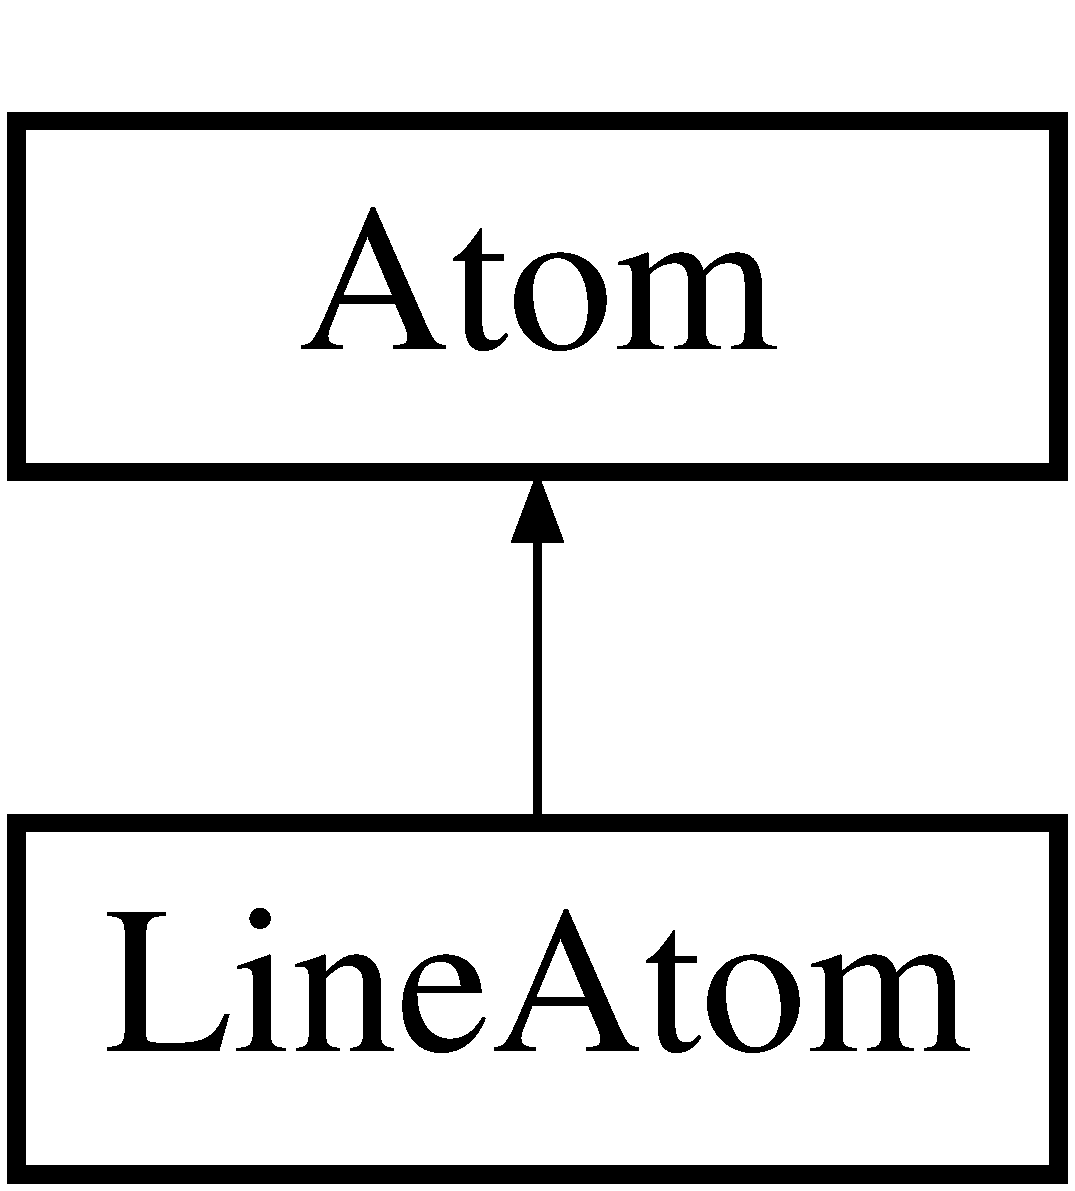
\includegraphics[height=2.000000cm]{class_line_atom}
\end{center}
\end{figure}
\subsection*{Public Member Functions}
\begin{DoxyCompactItemize}
\item 
\hypertarget{class_line_atom_abdf3de986b0d455cac39497e323898dc}{{\bfseries Line\-Atom} (float k\-P, float k\-I, float k\-D, C\-A\-N\-Jaguar $\ast$front\-Left, C\-A\-N\-Jaguar $\ast$rear\-Left, C\-A\-N\-Jaguar $\ast$front\-Right, C\-A\-N\-Jaguar $\ast$rear\-Right, float distance)}\label{class_line_atom_abdf3de986b0d455cac39497e323898dc}

\item 
\hypertarget{class_line_atom_a576d473b8fdd59aba7117529a69e37d0}{void {\bfseries Execute} ()}\label{class_line_atom_a576d473b8fdd59aba7117529a69e37d0}

\end{DoxyCompactItemize}
\subsection*{Additional Inherited Members}


The documentation for this class was generated from the following files\-:\begin{DoxyCompactItemize}
\item 
Varun\-\_\-\-Atoms/Atom.\-h\item 
Varun\-\_\-\-Atoms/Atom.\-cpp\end{DoxyCompactItemize}

\hypertarget{structlog_file}{\section{log\-File Struct Reference}
\label{structlog_file}\index{log\-File@{log\-File}}
}


{\ttfamily \#include $<$T\-K\-O\-Logging.\-h$>$}

\subsection*{Public Attributes}
\begin{DoxyCompactItemize}
\item 
bool \hyperlink{structlog_file_a4a069d00b4f684751ecba0c9625eeae6}{opened}
\item 
std\-::ofstream \hyperlink{structlog_file_a78d1ffa2264f3fcb04177e06803a9426}{fp}
\end{DoxyCompactItemize}


\subsection{Detailed Description}
You know you like structs! This is a struct for the logging file. 

\subsection{Member Data Documentation}
\hypertarget{structlog_file_a78d1ffa2264f3fcb04177e06803a9426}{\index{log\-File@{log\-File}!fp@{fp}}
\index{fp@{fp}!logFile@{log\-File}}
\subsubsection[{fp}]{\setlength{\rightskip}{0pt plus 5cm}std\-::ofstream log\-File\-::fp}}\label{structlog_file_a78d1ffa2264f3fcb04177e06803a9426}
ofstream fp. The file. \hypertarget{structlog_file_a4a069d00b4f684751ecba0c9625eeae6}{\index{log\-File@{log\-File}!opened@{opened}}
\index{opened@{opened}!logFile@{log\-File}}
\subsubsection[{opened}]{\setlength{\rightskip}{0pt plus 5cm}bool log\-File\-::opened}}\label{structlog_file_a4a069d00b4f684751ecba0c9625eeae6}
bool opened. Whether the file is open or not. 

The documentation for this struct was generated from the following files\-:\begin{DoxyCompactItemize}
\item 
Official\-Mark\-I\-X\-Code/T\-K\-O\-Logging.\-h\item 
Pleva\-\_\-\-Comp\-\_\-\-Logging/T\-K\-O\-Logging.\-h\end{DoxyCompactItemize}

\hypertarget{class_mark_i_x}{\section{Mark\-I\-X Class Reference}
\label{class_mark_i_x}\index{Mark\-I\-X@{Mark\-I\-X}}
}
\subsection*{Public Member Functions}
\begin{DoxyCompactItemize}
\item 
\hypertarget{class_mark_i_x_adca4ea1bab73e885b019e8cf1a5707fe}{void {\bfseries Disabled} ()}\label{class_mark_i_x_adca4ea1bab73e885b019e8cf1a5707fe}

\item 
\hypertarget{class_mark_i_x_aea97f16722f64241e523e413011bd814}{void {\bfseries Autonomous} (void)}\label{class_mark_i_x_aea97f16722f64241e523e413011bd814}

\item 
\hypertarget{class_mark_i_x_a8ddc43e1aab8dac7ca737f929507e22b}{void {\bfseries Operator\-Control} (void)}\label{class_mark_i_x_a8ddc43e1aab8dac7ca737f929507e22b}

\item 
\hypertarget{class_mark_i_x_afc1e96c6885d68a2a2eca02fe3e29de0}{void {\bfseries Driver} ()}\label{class_mark_i_x_afc1e96c6885d68a2a2eca02fe3e29de0}

\item 
\hypertarget{class_mark_i_x_aaaebc36ed027d8bc5f0a6f655be57879}{void {\bfseries Operator} ()}\label{class_mark_i_x_aaaebc36ed027d8bc5f0a6f655be57879}

\end{DoxyCompactItemize}


The documentation for this class was generated from the following file\-:\begin{DoxyCompactItemize}
\item 
Official\-Mark\-I\-X\-Code/Mark\-I\-X.\-cpp\end{DoxyCompactItemize}

\hypertarget{class_molecule}{\section{Molecule Class Reference}
\label{class_molecule}\index{Molecule@{Molecule}}
}
\subsection*{Public Member Functions}
\begin{DoxyCompactItemize}
\item 
\hypertarget{class_molecule_a90df5c5155c83ac1c3c2d7a52f733ede}{{\bfseries Molecule} (C\-A\-N\-Jaguar $\ast$front\-Left, C\-A\-N\-Jaguar $\ast$rear\-Left, C\-A\-N\-Jaguar $\ast$front\-Right, C\-A\-N\-Jaguar $\ast$rear\-Right, Gyro $\ast$gyro)}\label{class_molecule_a90df5c5155c83ac1c3c2d7a52f733ede}

\item 
\hypertarget{class_molecule_a859c25bb06ca6ad8a51dd63dab9a65f8}{void {\bfseries Add\-Line\-Atom} (float k\-P, float k\-I, float k\-D, float distance)}\label{class_molecule_a859c25bb06ca6ad8a51dd63dab9a65f8}

\item 
\hypertarget{class_molecule_a26a113923a688697923d32d8fd68676e}{void {\bfseries Add\-Turn\-Atom} (float k\-P, float k\-I, float k\-D, float angle)}\label{class_molecule_a26a113923a688697923d32d8fd68676e}

\item 
\hypertarget{class_molecule_a13d4f6b203fe789f6b0f00c691915d7f}{void {\bfseries Add\-Pause\-Atom} (float seconds)}\label{class_molecule_a13d4f6b203fe789f6b0f00c691915d7f}

\item 
\hypertarget{class_molecule_ae651169ec7e2da3f3108e7539c473554}{void {\bfseries Execute} ()}\label{class_molecule_ae651169ec7e2da3f3108e7539c473554}

\item 
\hypertarget{class_molecule_a2e6a136a2ffa52fb3b77e8cfa12cdad6}{bool {\bfseries Done} ()}\label{class_molecule_a2e6a136a2ffa52fb3b77e8cfa12cdad6}

\end{DoxyCompactItemize}


The documentation for this class was generated from the following files\-:\begin{DoxyCompactItemize}
\item 
Varun\-\_\-\-Atoms/Molecule.\-h\item 
Varun\-\_\-\-Atoms/Molecule.\-cpp\end{DoxyCompactItemize}

\hypertarget{class_pause_atom}{\section{Pause\-Atom Class Reference}
\label{class_pause_atom}\index{Pause\-Atom@{Pause\-Atom}}
}
Inheritance diagram for Pause\-Atom\-:\begin{figure}[H]
\begin{center}
\leavevmode
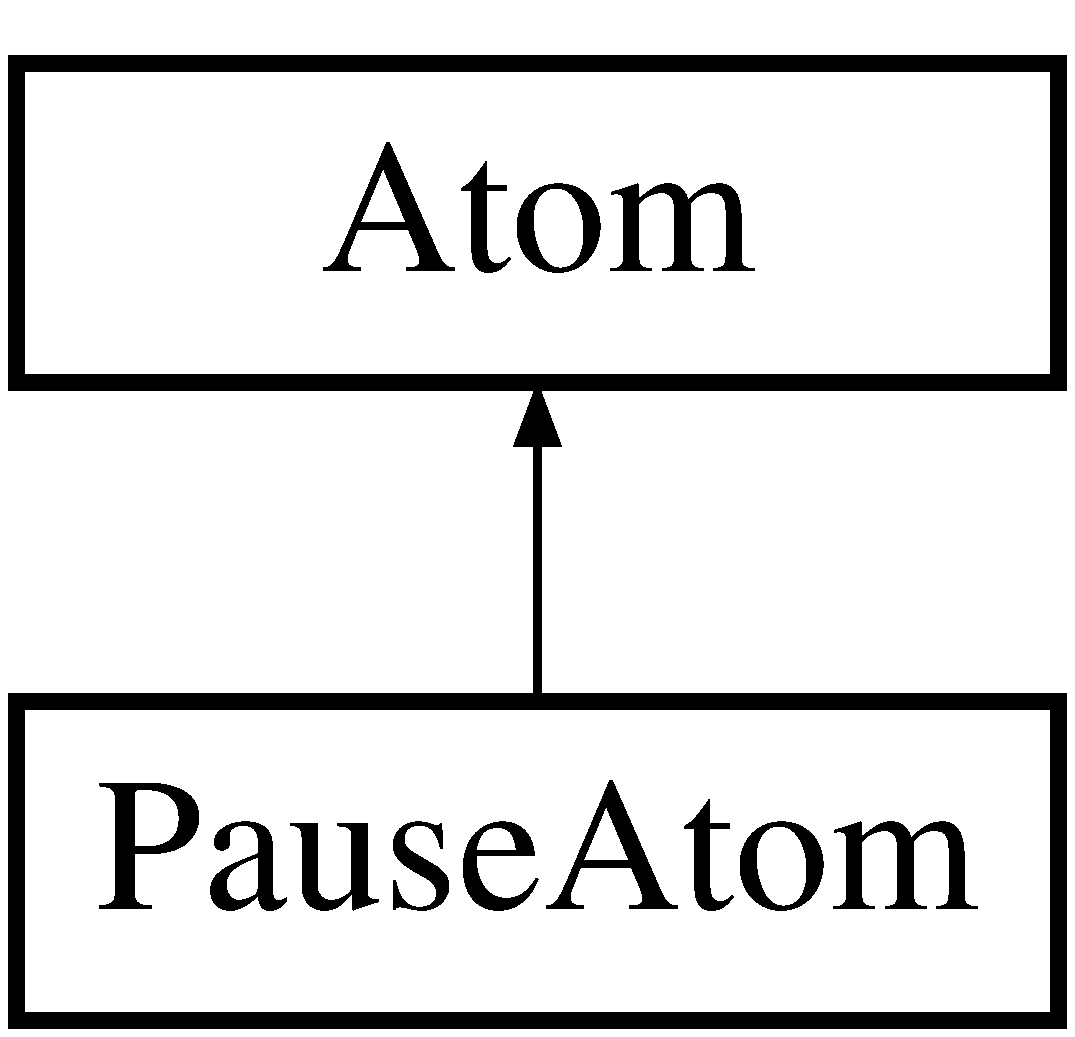
\includegraphics[height=2.000000cm]{class_pause_atom}
\end{center}
\end{figure}
\subsection*{Public Member Functions}
\begin{DoxyCompactItemize}
\item 
\hypertarget{class_pause_atom_a5d14b1d8911be8cf0155404b9b0358e5}{{\bfseries Pause\-Atom} (C\-A\-N\-Jaguar $\ast$front\-Left, C\-A\-N\-Jaguar $\ast$rear\-Left, C\-A\-N\-Jaguar $\ast$front\-Right, C\-A\-N\-Jaguar $\ast$rear\-Right, float seconds)}\label{class_pause_atom_a5d14b1d8911be8cf0155404b9b0358e5}

\item 
\hypertarget{class_pause_atom_aa2bf24fcd9b6c209101d256ad6735749}{void {\bfseries Execute} ()}\label{class_pause_atom_aa2bf24fcd9b6c209101d256ad6735749}

\end{DoxyCompactItemize}
\subsection*{Additional Inherited Members}


The documentation for this class was generated from the following files\-:\begin{DoxyCompactItemize}
\item 
Varun\-\_\-\-Atoms/Atom.\-h\item 
Varun\-\_\-\-Atoms/Atom.\-cpp\end{DoxyCompactItemize}

\hypertarget{class_pneumatic_controller}{\section{Pneumatic\-Controller Class Reference}
\label{class_pneumatic_controller}\index{Pneumatic\-Controller@{Pneumatic\-Controller}}
}
\subsection*{Public Member Functions}
\begin{DoxyCompactItemize}
\item 
\hypertarget{class_pneumatic_controller_acac78be574146f7965268a05550949d1}{{\bfseries Pneumatic\-Controller} (int port1, int port2, int port3)}\label{class_pneumatic_controller_acac78be574146f7965268a05550949d1}

\item 
\hypertarget{class_pneumatic_controller_a328609849a52748de3fb1b46a4ea0a82}{void {\bfseries Extend} ()}\label{class_pneumatic_controller_a328609849a52748de3fb1b46a4ea0a82}

\item 
\hypertarget{class_pneumatic_controller_a9cb7f96e438d830a0d3f2fb6bb256fe9}{void {\bfseries Retract} ()}\label{class_pneumatic_controller_a9cb7f96e438d830a0d3f2fb6bb256fe9}

\item 
\hypertarget{class_pneumatic_controller_acac78be574146f7965268a05550949d1}{{\bfseries Pneumatic\-Controller} (int port1, int port2, int port3)}\label{class_pneumatic_controller_acac78be574146f7965268a05550949d1}

\item 
\hypertarget{class_pneumatic_controller_a328609849a52748de3fb1b46a4ea0a82}{void {\bfseries Extend} ()}\label{class_pneumatic_controller_a328609849a52748de3fb1b46a4ea0a82}

\item 
\hypertarget{class_pneumatic_controller_a9cb7f96e438d830a0d3f2fb6bb256fe9}{void {\bfseries Retract} ()}\label{class_pneumatic_controller_a9cb7f96e438d830a0d3f2fb6bb256fe9}

\item 
\hypertarget{class_pneumatic_controller_a50e4aa1e4600c8d0741e9dbc05ec4c01}{Solenoid $\ast$ {\bfseries Get\-Solenoid} (int i)}\label{class_pneumatic_controller_a50e4aa1e4600c8d0741e9dbc05ec4c01}

\item 
\hypertarget{class_pneumatic_controller_a9bbc80dafd1575b43297d5ec10f99e1a}{bool {\bfseries Get\-State} ()}\label{class_pneumatic_controller_a9bbc80dafd1575b43297d5ec10f99e1a}

\end{DoxyCompactItemize}
\subsection*{Protected Attributes}
\begin{DoxyCompactItemize}
\item 
\hypertarget{class_pneumatic_controller_a1848c7ad0fe86fee27f407f14300ea1d}{Solenoid $\ast$ {\bfseries s} \mbox{[}2\mbox{]}}\label{class_pneumatic_controller_a1848c7ad0fe86fee27f407f14300ea1d}

\item 
\hypertarget{class_pneumatic_controller_aaf5da98ab6220bc3830e4f098392d725}{vector$<$ Solenoid $\ast$ $>$ $\ast$ {\bfseries s}}\label{class_pneumatic_controller_aaf5da98ab6220bc3830e4f098392d725}

\end{DoxyCompactItemize}


The documentation for this class was generated from the following files\-:\begin{DoxyCompactItemize}
\item 
Archived\-Controller\-Test/Pneumatic\-Controller.\-h\item 
Tanay\-\_\-\-Pneumatic\-Controller\-Test/Pneumatic\-Controller.\-h\item 
Archived\-Controller\-Test/Pneumatic\-Controller.\-cpp\item 
Tanay\-\_\-\-Pneumatic\-Controller\-Test/Pneumatic\-Controller.\-cpp\end{DoxyCompactItemize}

\hypertarget{class_pneumatics}{\section{Pneumatics Class Reference}
\label{class_pneumatics}\index{Pneumatics@{Pneumatics}}
}
\subsection*{Public Member Functions}
\begin{DoxyCompactItemize}
\item 
\hypertarget{class_pneumatics_a1b76e960a17e491d97ea7767ad2b389a}{{\bfseries Pneumatics} (int port1, int start, int end)}\label{class_pneumatics_a1b76e960a17e491d97ea7767ad2b389a}

\item 
\hypertarget{class_pneumatics_a82b412ea457d2eec590200d9dd04da19}{void {\bfseries Extend} (int num)}\label{class_pneumatics_a82b412ea457d2eec590200d9dd04da19}

\item 
\hypertarget{class_pneumatics_a21e16ac50d4963cb892243e1bf052f7a}{void {\bfseries Retract} (int num)}\label{class_pneumatics_a21e16ac50d4963cb892243e1bf052f7a}

\item 
\hypertarget{class_pneumatics_a69de5c31a4aba8e8b1527de4daffc3f4}{{\bfseries Pneumatics} (int port1, int start, int end, int compressch, int compressp)}\label{class_pneumatics_a69de5c31a4aba8e8b1527de4daffc3f4}

\item 
\hypertarget{class_pneumatics_a82b412ea457d2eec590200d9dd04da19}{void {\bfseries Extend} (int num)}\label{class_pneumatics_a82b412ea457d2eec590200d9dd04da19}

\item 
\hypertarget{class_pneumatics_a21e16ac50d4963cb892243e1bf052f7a}{void {\bfseries Retract} (int num)}\label{class_pneumatics_a21e16ac50d4963cb892243e1bf052f7a}

\item 
\hypertarget{class_pneumatics_a80c6272cbd91295533d9d23ff3da3196}{\hyperlink{class_pneumatic_controller}{Pneumatic\-Controller} {\bfseries Get\-Pneumatic\-Controller} (int i)}\label{class_pneumatics_a80c6272cbd91295533d9d23ff3da3196}

\item 
\hypertarget{class_pneumatics_ac09ac770e54942604c90cf7a0e13c4c4}{Solenoid $\ast$ {\bfseries Get\-Solenoid} (int i, int i2)}\label{class_pneumatics_ac09ac770e54942604c90cf7a0e13c4c4}

\item 
\hypertarget{class_pneumatics_ac5161f50f53ab9450416df347f5a359f}{bool {\bfseries Get\-State} (int i)}\label{class_pneumatics_ac5161f50f53ab9450416df347f5a359f}

\item 
\hypertarget{class_pneumatics_acdb72cee406f3c5a516cc74468738642}{void {\bfseries Stop\-Compressor} ()}\label{class_pneumatics_acdb72cee406f3c5a516cc74468738642}

\end{DoxyCompactItemize}


The documentation for this class was generated from the following files\-:\begin{DoxyCompactItemize}
\item 
Archived\-Controller\-Test/Pneumatics.\-h\item 
Tanay\-\_\-\-Pneumatic\-Controller\-Test/Pneumatics.\-h\item 
Archived\-Controller\-Test/Pneumatics.\-cpp\item 
Tanay\-\_\-\-Pneumatic\-Controller\-Test/Pneumatics.\-cpp\end{DoxyCompactItemize}

\hypertarget{class_pneumatic_test}{\section{Pneumatic\-Test Class Reference}
\label{class_pneumatic_test}\index{Pneumatic\-Test@{Pneumatic\-Test}}
}
\subsection*{Public Member Functions}
\begin{DoxyCompactItemize}
\item 
void \hyperlink{class_pneumatic_test_aedd0331dfee430545e6f77359c55f49c}{Autonomous} (void)
\item 
void \hyperlink{class_pneumatic_test_a66a59497cdbd504df462c8b2820617e8}{Operator\-Control} (void)
\item 
\hypertarget{class_pneumatic_test_afad611bfbbf3a85466d034bef3591bd1}{void {\bfseries Disabled} ()}\label{class_pneumatic_test_afad611bfbbf3a85466d034bef3591bd1}

\end{DoxyCompactItemize}


\subsection{Detailed Description}
This is a demo program showing the use of the Robot\-Base class. The Simple\-Robot class is the base of a robot application that will automatically call your Autonomous and Operator\-Control methods at the right time as controlled by the switches on the driver station or the field controls. 

\subsection{Member Function Documentation}
\hypertarget{class_pneumatic_test_aedd0331dfee430545e6f77359c55f49c}{\index{Pneumatic\-Test@{Pneumatic\-Test}!Autonomous@{Autonomous}}
\index{Autonomous@{Autonomous}!PneumaticTest@{Pneumatic\-Test}}
\subsubsection[{Autonomous}]{\setlength{\rightskip}{0pt plus 5cm}void Pneumatic\-Test\-::\-Autonomous (
\begin{DoxyParamCaption}
\item[{void}]{}
\end{DoxyParamCaption}
)\hspace{0.3cm}{\ttfamily [inline]}}}\label{class_pneumatic_test_aedd0331dfee430545e6f77359c55f49c}
Drive left \& right motors for 2 seconds then stop \hypertarget{class_pneumatic_test_a66a59497cdbd504df462c8b2820617e8}{\index{Pneumatic\-Test@{Pneumatic\-Test}!Operator\-Control@{Operator\-Control}}
\index{Operator\-Control@{Operator\-Control}!PneumaticTest@{Pneumatic\-Test}}
\subsubsection[{Operator\-Control}]{\setlength{\rightskip}{0pt plus 5cm}void Pneumatic\-Test\-::\-Operator\-Control (
\begin{DoxyParamCaption}
\item[{void}]{}
\end{DoxyParamCaption}
)\hspace{0.3cm}{\ttfamily [inline]}}}\label{class_pneumatic_test_a66a59497cdbd504df462c8b2820617e8}
Runs the motors with arcade steering. 

The documentation for this class was generated from the following file\-:\begin{DoxyCompactItemize}
\item 
Tanay\-\_\-\-Pneumatic\-Controller\-Test/My\-Robot.\-cpp\end{DoxyCompactItemize}

\hypertarget{class_robot_demo}{\section{Robot\-Demo Class Reference}
\label{class_robot_demo}\index{Robot\-Demo@{Robot\-Demo}}
}
\subsection*{Public Member Functions}
\begin{DoxyCompactItemize}
\item 
void \hyperlink{class_robot_demo_a80f9c6496e671ca2145d7f5543985e9a}{Autonomous} (void)
\item 
void \hyperlink{class_robot_demo_aea3d3a6789fa41653464bddc48d6a2c1}{Operator\-Control} (void)
\item 
\hypertarget{class_robot_demo_a80f9c6496e671ca2145d7f5543985e9a}{void {\bfseries Autonomous} (void)}\label{class_robot_demo_a80f9c6496e671ca2145d7f5543985e9a}

\item 
\hypertarget{class_robot_demo_aea3d3a6789fa41653464bddc48d6a2c1}{void {\bfseries Operator\-Control} (void)}\label{class_robot_demo_aea3d3a6789fa41653464bddc48d6a2c1}

\item 
\hypertarget{class_robot_demo_a6974abdcd125a7701b6227d7de3794ea}{bool {\bfseries pixel\-In\-R\-G\-B\-Threshold} (R\-G\-B\-Value $\ast$pixel, Threshold \&threshold)}\label{class_robot_demo_a6974abdcd125a7701b6227d7de3794ea}

\item 
\hypertarget{class_robot_demo_a39d5d27c5c76c0a5482b24650bf85fb4}{void {\bfseries Get\-Starting\-Point} (int \&starting\-X, int \&starting\-Y, Image\-Info \&info, Rect \&bounding\-Rect, Threshold \&threshold, bool left\-Side)}\label{class_robot_demo_a39d5d27c5c76c0a5482b24650bf85fb4}

\item 
\hypertarget{class_robot_demo_a7d420e946e4e7ff2e61bd1da01b129dc}{int {\bfseries Find\-Corner} (Threshold \&threshold, Image\-Info \&info, int starting\-X, int starting\-Y, bool left\-Side, bool top\-Corner)}\label{class_robot_demo_a7d420e946e4e7ff2e61bd1da01b129dc}

\item 
\hypertarget{class_robot_demo_a3b3c94e56982e70da6883c71d4cd5bb9}{void {\bfseries Disabled} ()}\label{class_robot_demo_a3b3c94e56982e70da6883c71d4cd5bb9}

\item 
\hypertarget{class_robot_demo_aea3d3a6789fa41653464bddc48d6a2c1}{void {\bfseries Operator\-Control} (void)}\label{class_robot_demo_aea3d3a6789fa41653464bddc48d6a2c1}

\item 
void \hyperlink{class_robot_demo_a80f9c6496e671ca2145d7f5543985e9a}{Autonomous} (void)
\item 
void \hyperlink{class_robot_demo_aea3d3a6789fa41653464bddc48d6a2c1}{Operator\-Control} (void)
\item 
\hypertarget{class_robot_demo_a159d7d19b1eb3c1489561d101f209112}{float {\bfseries Calculate\-Velocity} (float dist, float height, float theta)}\label{class_robot_demo_a159d7d19b1eb3c1489561d101f209112}

\item 
void \hyperlink{class_robot_demo_a80f9c6496e671ca2145d7f5543985e9a}{Autonomous} (void)
\item 
float \hyperlink{class_robot_demo_af24ec862633fd0927a00d492c32f2cf5}{Analyze\-Gyro\-Angle} (\hyperlink{class_t_k_o_gyro}{T\-K\-O\-Gyro} \&gyro)
\item 
\hypertarget{class_robot_demo_aea3d3a6789fa41653464bddc48d6a2c1}{void {\bfseries Operator\-Control} (void)}\label{class_robot_demo_aea3d3a6789fa41653464bddc48d6a2c1}

\item 
\hypertarget{class_robot_demo_ae8affaa7a9f2b4b4952187282ab3ff60}{void {\bfseries Auto\-Balance} (void)}\label{class_robot_demo_ae8affaa7a9f2b4b4952187282ab3ff60}

\item 
\hypertarget{class_robot_demo_a6d678cd2412907db5c2b62c57257b229}{void {\bfseries End\-Auto\-Balance} (void)}\label{class_robot_demo_a6d678cd2412907db5c2b62c57257b229}

\item 
\hypertarget{class_robot_demo_a80f9c6496e671ca2145d7f5543985e9a}{void {\bfseries Autonomous} (void)}\label{class_robot_demo_a80f9c6496e671ca2145d7f5543985e9a}

\item 
\hypertarget{class_robot_demo_aea3d3a6789fa41653464bddc48d6a2c1}{void {\bfseries Operator\-Control} (void)}\label{class_robot_demo_aea3d3a6789fa41653464bddc48d6a2c1}

\item 
\hypertarget{class_robot_demo_a97242890ba9107422e5af04bcb96cdff}{void {\bfseries Robot\-Init} (void)}\label{class_robot_demo_a97242890ba9107422e5af04bcb96cdff}

\item 
\hypertarget{class_robot_demo_aea3d3a6789fa41653464bddc48d6a2c1}{void {\bfseries Operator\-Control} (void)}\label{class_robot_demo_aea3d3a6789fa41653464bddc48d6a2c1}

\item 
\hypertarget{class_robot_demo_a80f9c6496e671ca2145d7f5543985e9a}{void {\bfseries Autonomous} (void)}\label{class_robot_demo_a80f9c6496e671ca2145d7f5543985e9a}

\item 
\hypertarget{class_robot_demo_aea3d3a6789fa41653464bddc48d6a2c1}{void {\bfseries Operator\-Control} (void)}\label{class_robot_demo_aea3d3a6789fa41653464bddc48d6a2c1}

\end{DoxyCompactItemize}


\subsection{Detailed Description}
This is a demo program showing the use of the Robot\-Base class. The Simple\-Robot class is the base of a robot application that will automatically call your Autonomous and Operator\-Control methods at the right time as controlled by the switches on the driver station or the field controls. 

\subsection{Member Function Documentation}
\hypertarget{class_robot_demo_af24ec862633fd0927a00d492c32f2cf5}{\index{Robot\-Demo@{Robot\-Demo}!Analyze\-Gyro\-Angle@{Analyze\-Gyro\-Angle}}
\index{Analyze\-Gyro\-Angle@{Analyze\-Gyro\-Angle}!RobotDemo@{Robot\-Demo}}
\subsubsection[{Analyze\-Gyro\-Angle}]{\setlength{\rightskip}{0pt plus 5cm}float Robot\-Demo\-::\-Analyze\-Gyro\-Angle (
\begin{DoxyParamCaption}
\item[{{\bf T\-K\-O\-Gyro} \&}]{gyro}
\end{DoxyParamCaption}
)\hspace{0.3cm}{\ttfamily [inline]}}}\label{class_robot_demo_af24ec862633fd0927a00d492c32f2cf5}
Runs the motors with arcade steering. \hypertarget{class_robot_demo_a80f9c6496e671ca2145d7f5543985e9a}{\index{Robot\-Demo@{Robot\-Demo}!Autonomous@{Autonomous}}
\index{Autonomous@{Autonomous}!RobotDemo@{Robot\-Demo}}
\subsubsection[{Autonomous}]{\setlength{\rightskip}{0pt plus 5cm}void Robot\-Demo\-::\-Autonomous (
\begin{DoxyParamCaption}
\item[{void}]{}
\end{DoxyParamCaption}
)\hspace{0.3cm}{\ttfamily [inline]}}}\label{class_robot_demo_a80f9c6496e671ca2145d7f5543985e9a}
Drive left \& right motors for 2 seconds then stop \hypertarget{class_robot_demo_a80f9c6496e671ca2145d7f5543985e9a}{\index{Robot\-Demo@{Robot\-Demo}!Autonomous@{Autonomous}}
\index{Autonomous@{Autonomous}!RobotDemo@{Robot\-Demo}}
\subsubsection[{Autonomous}]{\setlength{\rightskip}{0pt plus 5cm}void Robot\-Demo\-::\-Autonomous (
\begin{DoxyParamCaption}
\item[{void}]{}
\end{DoxyParamCaption}
)\hspace{0.3cm}{\ttfamily [inline]}}}\label{class_robot_demo_a80f9c6496e671ca2145d7f5543985e9a}
Drive left \& right motors for 2 seconds then stop \hypertarget{class_robot_demo_a80f9c6496e671ca2145d7f5543985e9a}{\index{Robot\-Demo@{Robot\-Demo}!Autonomous@{Autonomous}}
\index{Autonomous@{Autonomous}!RobotDemo@{Robot\-Demo}}
\subsubsection[{Autonomous}]{\setlength{\rightskip}{0pt plus 5cm}void Robot\-Demo\-::\-Autonomous (
\begin{DoxyParamCaption}
\item[{void}]{}
\end{DoxyParamCaption}
)\hspace{0.3cm}{\ttfamily [inline]}}}\label{class_robot_demo_a80f9c6496e671ca2145d7f5543985e9a}
Drive left \& right motors for 2 seconds then stop \hypertarget{class_robot_demo_aea3d3a6789fa41653464bddc48d6a2c1}{\index{Robot\-Demo@{Robot\-Demo}!Operator\-Control@{Operator\-Control}}
\index{Operator\-Control@{Operator\-Control}!RobotDemo@{Robot\-Demo}}
\subsubsection[{Operator\-Control}]{\setlength{\rightskip}{0pt plus 5cm}void Robot\-Demo\-::\-Operator\-Control (
\begin{DoxyParamCaption}
\item[{void}]{}
\end{DoxyParamCaption}
)\hspace{0.3cm}{\ttfamily [inline]}}}\label{class_robot_demo_aea3d3a6789fa41653464bddc48d6a2c1}
Runs the motors with arcade steering. \hypertarget{class_robot_demo_aea3d3a6789fa41653464bddc48d6a2c1}{\index{Robot\-Demo@{Robot\-Demo}!Operator\-Control@{Operator\-Control}}
\index{Operator\-Control@{Operator\-Control}!RobotDemo@{Robot\-Demo}}
\subsubsection[{Operator\-Control}]{\setlength{\rightskip}{0pt plus 5cm}void Robot\-Demo\-::\-Operator\-Control (
\begin{DoxyParamCaption}
\item[{void}]{}
\end{DoxyParamCaption}
)\hspace{0.3cm}{\ttfamily [inline]}}}\label{class_robot_demo_aea3d3a6789fa41653464bddc48d6a2c1}
Runs the motors with arcade steering. 

The documentation for this class was generated from the following files\-:\begin{DoxyCompactItemize}
\item 
Archived\-Controller\-Test/My\-Robot.\-cpp\item 
Mark\-I\-X\-\_\-\-Varun\-\_\-\-Ship\-\_\-\-Day/My\-Robot.\-cpp\item 
Mark\-I\-X\-\_\-\-Varun\-\_\-\-Vision/Vision.\-cpp\item 
Sonar\-Testing/My\-Robot.\-cpp\item 
Vadim\-\_\-brandi\-\_\-autobalance/Mark\-I\-X.\-cpp\item 
Varun\-\_\-\-Atoms/My\-Robot.\-cpp\item 
Varun\-\_\-\-Joystick/My\-Robot.\-cpp\item 
Varun\-\_\-\-Shooter\-\_\-\-Heavily\-Commented/My\-Robot.\-cpp\end{DoxyCompactItemize}

\hypertarget{class_shoot_atom}{\section{Shoot\-Atom Class Reference}
\label{class_shoot_atom}\index{Shoot\-Atom@{Shoot\-Atom}}
}
Inheritance diagram for Shoot\-Atom\-:\begin{figure}[H]
\begin{center}
\leavevmode
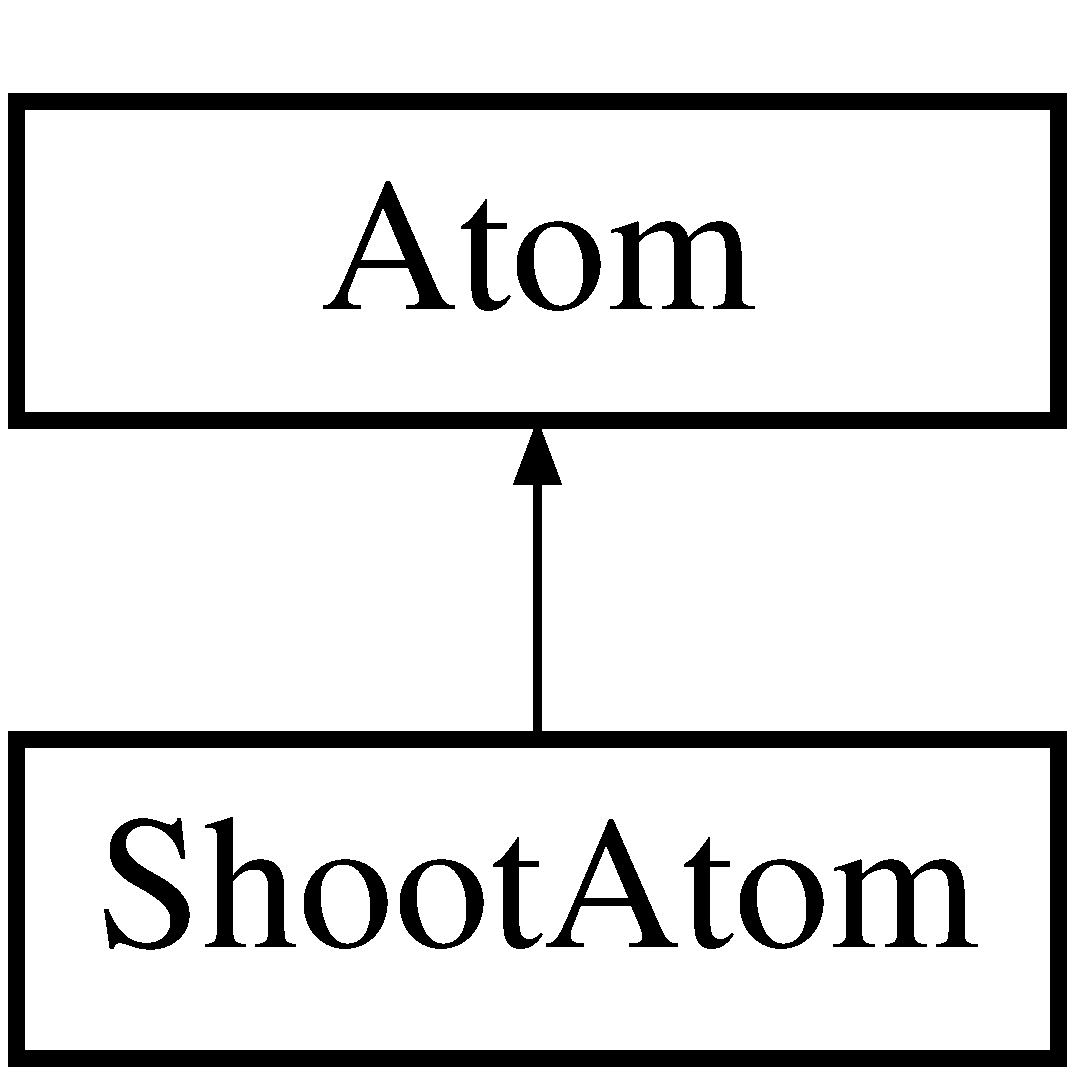
\includegraphics[height=2.000000cm]{class_shoot_atom}
\end{center}
\end{figure}
\subsection*{Public Member Functions}
\begin{DoxyCompactItemize}
\item 
\hypertarget{class_shoot_atom_a8eed14486140f0a16973244e78a6855e}{{\bfseries Shoot\-Atom} (C\-A\-N\-Jaguar $\ast$front\-Left, C\-A\-N\-Jaguar $\ast$rear\-Left, C\-A\-N\-Jaguar $\ast$front\-Right, C\-A\-N\-Jaguar $\ast$rear\-Right)}\label{class_shoot_atom_a8eed14486140f0a16973244e78a6855e}

\item 
\hypertarget{class_shoot_atom_a741db2f29645dd5521f94265b8d2fa73}{void {\bfseries Execute} ()}\label{class_shoot_atom_a741db2f29645dd5521f94265b8d2fa73}

\end{DoxyCompactItemize}
\subsection*{Additional Inherited Members}


The documentation for this class was generated from the following files\-:\begin{DoxyCompactItemize}
\item 
Varun\-\_\-\-Atoms/Atom.\-h\item 
Varun\-\_\-\-Atoms/Atom.\-cpp\end{DoxyCompactItemize}

\hypertarget{class_task_test}{\section{Task\-Test Class Reference}
\label{class_task_test}\index{Task\-Test@{Task\-Test}}
}
\subsection*{Public Member Functions}
\begin{DoxyCompactItemize}
\item 
void \hyperlink{class_task_test_a8680eee6f9af558b8b94a0328d186217}{Autonomous} (void)
\item 
void \hyperlink{class_task_test_a05a602d8807acb207c86825deab3b9d1}{Operator\-Control} (void)
\item 
\hypertarget{class_task_test_a83b7f12433df44c032fc4a2dac4ddbb6}{void {\bfseries Lock} ()}\label{class_task_test_a83b7f12433df44c032fc4a2dac4ddbb6}

\item 
\hypertarget{class_task_test_aa34bdc5d2ae91c7de1afc4d2dfe7aa48}{void {\bfseries Unlock} ()}\label{class_task_test_aa34bdc5d2ae91c7de1afc4d2dfe7aa48}

\item 
\hypertarget{class_task_test_a0917f09429234595d076ef19a2753935}{void {\bfseries Switchto\-Arcade\-Drive} ()}\label{class_task_test_a0917f09429234595d076ef19a2753935}

\item 
\hypertarget{class_task_test_aab9af5da7a3c000e9678c0a0f40f81ec}{void {\bfseries Switchto\-Tank\-Drive} ()}\label{class_task_test_aab9af5da7a3c000e9678c0a0f40f81ec}

\end{DoxyCompactItemize}


\subsection{Detailed Description}
This is a demo program showing the use of the Robot\-Base class. The Simple\-Robot class is the base of a robot application that will automatically call your Autonomous and Operator\-Control methods at the right time as controlled by the switches on the driver station or the field controls. 

\subsection{Member Function Documentation}
\hypertarget{class_task_test_a8680eee6f9af558b8b94a0328d186217}{\index{Task\-Test@{Task\-Test}!Autonomous@{Autonomous}}
\index{Autonomous@{Autonomous}!TaskTest@{Task\-Test}}
\subsubsection[{Autonomous}]{\setlength{\rightskip}{0pt plus 5cm}void Task\-Test\-::\-Autonomous (
\begin{DoxyParamCaption}
\item[{void}]{}
\end{DoxyParamCaption}
)\hspace{0.3cm}{\ttfamily [inline]}}}\label{class_task_test_a8680eee6f9af558b8b94a0328d186217}
Drive left \& right motors for 2 seconds then stop \hypertarget{class_task_test_a05a602d8807acb207c86825deab3b9d1}{\index{Task\-Test@{Task\-Test}!Operator\-Control@{Operator\-Control}}
\index{Operator\-Control@{Operator\-Control}!TaskTest@{Task\-Test}}
\subsubsection[{Operator\-Control}]{\setlength{\rightskip}{0pt plus 5cm}void Task\-Test\-::\-Operator\-Control (
\begin{DoxyParamCaption}
\item[{void}]{}
\end{DoxyParamCaption}
)\hspace{0.3cm}{\ttfamily [inline]}}}\label{class_task_test_a05a602d8807acb207c86825deab3b9d1}
Runs the motors with arcade steering. 

The documentation for this class was generated from the following file\-:\begin{DoxyCompactItemize}
\item 
Tanay\-\_\-\-Task\-Testing/My\-Robot.\-cpp\end{DoxyCompactItemize}

\hypertarget{class_testing}{\section{Testing Class Reference}
\label{class_testing}\index{Testing@{Testing}}
}
\subsection*{Public Member Functions}
\begin{DoxyCompactItemize}
\item 
\hypertarget{class_testing_a7d268d698c9a059466eb74a8bf356652}{void {\bfseries Autonomous} (void)}\label{class_testing_a7d268d698c9a059466eb74a8bf356652}

\item 
\hypertarget{class_testing_a0f1036b6176326cd3d1c43d717635567}{void {\bfseries Operator\-Control} (void)}\label{class_testing_a0f1036b6176326cd3d1c43d717635567}

\end{DoxyCompactItemize}


The documentation for this class was generated from the following file\-:\begin{DoxyCompactItemize}
\item 
Mark\-I\-X\-\_\-\-Varun\-\_\-\-Conveyor/Testing.\-cpp\end{DoxyCompactItemize}

\hypertarget{class_t_k_o_camera}{\section{T\-K\-O\-Camera Class Reference}
\label{class_t_k_o_camera}\index{T\-K\-O\-Camera@{T\-K\-O\-Camera}}
}
\subsection*{Public Member Functions}
\begin{DoxyCompactItemize}
\item 
\hypertarget{class_t_k_o_camera_a6f548d053fbb799924b99e5795addbdb}{double {\bfseries P\-I\-D\-Get} ()}\label{class_t_k_o_camera_a6f548d053fbb799924b99e5795addbdb}

\item 
\hypertarget{class_t_k_o_camera_af13110a52d21c440ceab5bdf2cb6de59}{float {\bfseries Get\-Angle} ()}\label{class_t_k_o_camera_af13110a52d21c440ceab5bdf2cb6de59}

\end{DoxyCompactItemize}


The documentation for this class was generated from the following files\-:\begin{DoxyCompactItemize}
\item 
Mark\-I\-X\-\_\-\-Varun\-\_\-\-Vision/T\-K\-O\-Camera.\-h\item 
Tanay\-\_\-\-Auto\-Targetting/T\-K\-O\-Camera.\-h\item 
Mark\-I\-X\-\_\-\-Varun\-\_\-\-Vision/T\-K\-O\-Camera.\-cpp\item 
Tanay\-\_\-\-Auto\-Targetting/T\-K\-O\-Camera.\-cpp\end{DoxyCompactItemize}

\hypertarget{class_t_k_o_conveyor}{\section{T\-K\-O\-Conveyor Class Reference}
\label{class_t_k_o_conveyor}\index{T\-K\-O\-Conveyor@{T\-K\-O\-Conveyor}}
}
\subsection*{Public Member Functions}
\begin{DoxyCompactItemize}
\item 
\hypertarget{class_t_k_o_conveyor_a06d6adff52d9b77308ed1d29f47b1bf8}{void {\bfseries Run} (bool shoot\-Button, bool can\-Shoot)}\label{class_t_k_o_conveyor_a06d6adff52d9b77308ed1d29f47b1bf8}

\item 
\hypertarget{class_t_k_o_conveyor_a8fe70dce57a1e7e7124177cc9413dbd3}{bool {\bfseries Stuff} ()}\label{class_t_k_o_conveyor_a8fe70dce57a1e7e7124177cc9413dbd3}

\item 
\hypertarget{class_t_k_o_conveyor_a68d6a4bdf4c7f640da4977366c2e6add}{{\bfseries T\-K\-O\-Conveyor} (int port1=3, int port2=2, int port3=1, int port4=2, int port5=1)}\label{class_t_k_o_conveyor_a68d6a4bdf4c7f640da4977366c2e6add}

\item 
\hypertarget{class_t_k_o_conveyor_ac46547907a0ff74117d63e134d1c5985}{void {\bfseries Run} (bool can\-Shoot)}\label{class_t_k_o_conveyor_ac46547907a0ff74117d63e134d1c5985}

\item 
\hypertarget{class_t_k_o_conveyor_aabaebf6851e31ec3c258534441aeb814}{void {\bfseries Override\-All} ()}\label{class_t_k_o_conveyor_aabaebf6851e31ec3c258534441aeb814}

\item 
\hypertarget{class_t_k_o_conveyor_ab998b5ba247e2dc337f01840cc6ade2f}{bool {\bfseries Can\-Enable\-Intake} ()}\label{class_t_k_o_conveyor_ab998b5ba247e2dc337f01840cc6ade2f}

\item 
\hypertarget{class_t_k_o_conveyor_adf4e54d355bc30f1da5a822cdecece12}{void {\bfseries End\-All} ()}\label{class_t_k_o_conveyor_adf4e54d355bc30f1da5a822cdecece12}

\item 
\hypertarget{class_t_k_o_conveyor_a7ed68e1b021a999dda718f02ea28c7ef}{void {\bfseries Reverse} ()}\label{class_t_k_o_conveyor_a7ed68e1b021a999dda718f02ea28c7ef}

\item 
\hypertarget{class_t_k_o_conveyor_a8d06cb72e39a9f8da636f0556b4ffd90}{int {\bfseries Get\-Num\-Balls} ()}\label{class_t_k_o_conveyor_a8d06cb72e39a9f8da636f0556b4ffd90}

\end{DoxyCompactItemize}


The documentation for this class was generated from the following files\-:\begin{DoxyCompactItemize}
\item 
Mark\-I\-X\-\_\-\-Varun\-\_\-\-Conveyor/T\-K\-O\-Conveyor.\-h\item 
Official\-Mark\-I\-X\-Code/T\-K\-O\-Conveyor.\-h\item 
Mark\-I\-X\-\_\-\-Varun\-\_\-\-Conveyor/T\-K\-O\-Conveyor.\-cpp\item 
Official\-Mark\-I\-X\-Code/T\-K\-O\-Conveyor.\-cpp\end{DoxyCompactItemize}

\hypertarget{class_t_k_o_gyro}{\section{T\-K\-O\-Gyro Class Reference}
\label{class_t_k_o_gyro}\index{T\-K\-O\-Gyro@{T\-K\-O\-Gyro}}
}


{\ttfamily \#include $<$T\-K\-O\-Gyro.\-h$>$}

\subsection*{Public Member Functions}
\begin{DoxyCompactItemize}
\item 
\hyperlink{class_t_k_o_gyro_a38334c169e97dceb6457e989875e93de}{T\-K\-O\-Gyro} (U\-I\-N\-T8 module\-Number, U\-I\-N\-T32 channel)
\item 
\hyperlink{class_t_k_o_gyro_a329cee1199b0935e646591c548e3502a}{T\-K\-O\-Gyro} (U\-I\-N\-T32 channel)
\item 
\hyperlink{class_t_k_o_gyro_ae4b751a9be6ae337957b20e3c3083e37}{T\-K\-O\-Gyro} (Analog\-Channel $\ast$channel)
\item 
\hypertarget{class_t_k_o_gyro_add8212e066db0ef3f2bdd01a9d01bb14}{{\bfseries T\-K\-O\-Gyro} (Analog\-Channel \&channel)}\label{class_t_k_o_gyro_add8212e066db0ef3f2bdd01a9d01bb14}

\item 
virtual \hyperlink{class_t_k_o_gyro_a0a59a50d0805a6f98a507933f77ed037}{$\sim$\-T\-K\-O\-Gyro} ()
\item 
virtual float \hyperlink{class_t_k_o_gyro_af2f5666e5f5d2402ecec2ac87613dc8c}{Get\-Angle} ()
\item 
void \hyperlink{class_t_k_o_gyro_a3b1296faa69e1175d3241f002edbb45e}{Set\-Sensitivity} (float volts\-Per\-Degree\-Per\-Second)
\item 
virtual void \hyperlink{class_t_k_o_gyro_a8d52b80879305a98620be59a5e089b64}{Reset} ()
\item 
double \hyperlink{class_t_k_o_gyro_ae5ab4261974fea729d252dbdad78326a}{P\-I\-D\-Get} ()
\end{DoxyCompactItemize}
\subsection*{Static Public Attributes}
\begin{DoxyCompactItemize}
\item 
\hypertarget{class_t_k_o_gyro_a794fe010f1390eb92d175ce8ace372fd}{static const U\-I\-N\-T32 {\bfseries k\-Oversample\-Bits} = 10}\label{class_t_k_o_gyro_a794fe010f1390eb92d175ce8ace372fd}

\item 
\hypertarget{class_t_k_o_gyro_a52e7e66f6fcdc4f9f34c0de39d88e427}{static const U\-I\-N\-T32 {\bfseries k\-Average\-Bits} = 0}\label{class_t_k_o_gyro_a52e7e66f6fcdc4f9f34c0de39d88e427}

\item 
\hypertarget{class_t_k_o_gyro_aa6e80a68440185d245310d30e714a9c7}{static const float {\bfseries k\-Samples\-Per\-Second} = 1000.\-0}\label{class_t_k_o_gyro_aa6e80a68440185d245310d30e714a9c7}

\item 
\hypertarget{class_t_k_o_gyro_a0c74698b86f1125fac52fc9d3e2d4bf2}{static const float {\bfseries k\-Calibration\-Sample\-Time} = 5.\-0}\label{class_t_k_o_gyro_a0c74698b86f1125fac52fc9d3e2d4bf2}

\item 
\hypertarget{class_t_k_o_gyro_aeb705e001e8af34a337ca38d178f386d}{static const float {\bfseries k\-Default\-Volts\-Per\-Degree\-Per\-Second} = 0.\-007}\label{class_t_k_o_gyro_aeb705e001e8af34a337ca38d178f386d}

\end{DoxyCompactItemize}


\subsection{Detailed Description}
Use a rate \hyperlink{class_t_k_o_gyro}{T\-K\-O\-Gyro} to return the robots heading relative to a starting position. The \hyperlink{class_t_k_o_gyro}{T\-K\-O\-Gyro} class tracks the robots heading based on the starting position. As the robot rotates the new heading is computed by integrating the rate of rotation returned by the sensor. When the class is instantiated, it does a short calibration routine where it samples the \hyperlink{class_t_k_o_gyro}{T\-K\-O\-Gyro} while at rest to determine the default offset. This is subtracted from each sample to determine the heading. This \hyperlink{class_t_k_o_gyro}{T\-K\-O\-Gyro} class must be used with a channel that is assigned one of the Analog accumulators from the F\-P\-G\-A. See Analog\-Channel for the current accumulator assignments. 

\subsection{Constructor \& Destructor Documentation}
\hypertarget{class_t_k_o_gyro_a38334c169e97dceb6457e989875e93de}{\index{T\-K\-O\-Gyro@{T\-K\-O\-Gyro}!T\-K\-O\-Gyro@{T\-K\-O\-Gyro}}
\index{T\-K\-O\-Gyro@{T\-K\-O\-Gyro}!TKOGyro@{T\-K\-O\-Gyro}}
\subsubsection[{T\-K\-O\-Gyro}]{\setlength{\rightskip}{0pt plus 5cm}T\-K\-O\-Gyro\-::\-T\-K\-O\-Gyro (
\begin{DoxyParamCaption}
\item[{U\-I\-N\-T8}]{module\-Number, }
\item[{U\-I\-N\-T32}]{channel}
\end{DoxyParamCaption}
)}}\label{class_t_k_o_gyro_a38334c169e97dceb6457e989875e93de}
\hyperlink{class_t_k_o_gyro}{T\-K\-O\-Gyro} constructor given a slot and a channel.


\begin{DoxyParams}{Parameters}
{\em module\-Number} & The analog module the \hyperlink{class_t_k_o_gyro}{T\-K\-O\-Gyro} is connected to (1). \\
\hline
{\em channel} & The analog channel the \hyperlink{class_t_k_o_gyro}{T\-K\-O\-Gyro} is connected to (1 or 2). \\
\hline
\end{DoxyParams}
\hypertarget{class_t_k_o_gyro_a329cee1199b0935e646591c548e3502a}{\index{T\-K\-O\-Gyro@{T\-K\-O\-Gyro}!T\-K\-O\-Gyro@{T\-K\-O\-Gyro}}
\index{T\-K\-O\-Gyro@{T\-K\-O\-Gyro}!TKOGyro@{T\-K\-O\-Gyro}}
\subsubsection[{T\-K\-O\-Gyro}]{\setlength{\rightskip}{0pt plus 5cm}T\-K\-O\-Gyro\-::\-T\-K\-O\-Gyro (
\begin{DoxyParamCaption}
\item[{U\-I\-N\-T32}]{channel}
\end{DoxyParamCaption}
)\hspace{0.3cm}{\ttfamily [explicit]}}}\label{class_t_k_o_gyro_a329cee1199b0935e646591c548e3502a}
\hyperlink{class_t_k_o_gyro}{T\-K\-O\-Gyro} constructor with only a channel.

Use the default analog module slot.


\begin{DoxyParams}{Parameters}
{\em channel} & The analog channel the \hyperlink{class_t_k_o_gyro}{T\-K\-O\-Gyro} is connected to. \\
\hline
\end{DoxyParams}
\hypertarget{class_t_k_o_gyro_ae4b751a9be6ae337957b20e3c3083e37}{\index{T\-K\-O\-Gyro@{T\-K\-O\-Gyro}!T\-K\-O\-Gyro@{T\-K\-O\-Gyro}}
\index{T\-K\-O\-Gyro@{T\-K\-O\-Gyro}!TKOGyro@{T\-K\-O\-Gyro}}
\subsubsection[{T\-K\-O\-Gyro}]{\setlength{\rightskip}{0pt plus 5cm}T\-K\-O\-Gyro\-::\-T\-K\-O\-Gyro (
\begin{DoxyParamCaption}
\item[{Analog\-Channel $\ast$}]{channel}
\end{DoxyParamCaption}
)\hspace{0.3cm}{\ttfamily [explicit]}}}\label{class_t_k_o_gyro_ae4b751a9be6ae337957b20e3c3083e37}
\hyperlink{class_t_k_o_gyro}{T\-K\-O\-Gyro} constructor with a precreated analog channel object. Use this constructor when the analog channel needs to be shared. There is no reference counting when an Analog\-Channel is passed to the \hyperlink{class_t_k_o_gyro}{T\-K\-O\-Gyro}. 
\begin{DoxyParams}{Parameters}
{\em channel} & The Analog\-Channel object that the \hyperlink{class_t_k_o_gyro}{T\-K\-O\-Gyro} is connected to. \\
\hline
\end{DoxyParams}
\hypertarget{class_t_k_o_gyro_a0a59a50d0805a6f98a507933f77ed037}{\index{T\-K\-O\-Gyro@{T\-K\-O\-Gyro}!$\sim$\-T\-K\-O\-Gyro@{$\sim$\-T\-K\-O\-Gyro}}
\index{$\sim$\-T\-K\-O\-Gyro@{$\sim$\-T\-K\-O\-Gyro}!TKOGyro@{T\-K\-O\-Gyro}}
\subsubsection[{$\sim$\-T\-K\-O\-Gyro}]{\setlength{\rightskip}{0pt plus 5cm}T\-K\-O\-Gyro\-::$\sim$\-T\-K\-O\-Gyro (
\begin{DoxyParamCaption}
{}
\end{DoxyParamCaption}
)\hspace{0.3cm}{\ttfamily [virtual]}}}\label{class_t_k_o_gyro_a0a59a50d0805a6f98a507933f77ed037}
Delete (free) the accumulator and the analog components used for the \hyperlink{class_t_k_o_gyro}{T\-K\-O\-Gyro}. 

\subsection{Member Function Documentation}
\hypertarget{class_t_k_o_gyro_af2f5666e5f5d2402ecec2ac87613dc8c}{\index{T\-K\-O\-Gyro@{T\-K\-O\-Gyro}!Get\-Angle@{Get\-Angle}}
\index{Get\-Angle@{Get\-Angle}!TKOGyro@{T\-K\-O\-Gyro}}
\subsubsection[{Get\-Angle}]{\setlength{\rightskip}{0pt plus 5cm}float T\-K\-O\-Gyro\-::\-Get\-Angle (
\begin{DoxyParamCaption}
\item[{void}]{}
\end{DoxyParamCaption}
)\hspace{0.3cm}{\ttfamily [virtual]}}}\label{class_t_k_o_gyro_af2f5666e5f5d2402ecec2ac87613dc8c}
Return the actual angle in degrees that the robot is currently facing.

The angle is based on the current accumulator value corrected by the oversampling rate, the \hyperlink{class_t_k_o_gyro}{T\-K\-O\-Gyro} type and the A/\-D calibration values. The angle is continuous, that is can go beyond 360 degrees. This make algorithms that wouldn't want to see a discontinuity in the \hyperlink{class_t_k_o_gyro}{T\-K\-O\-Gyro} output as it sweeps past 0 on the second time around.

\begin{DoxyReturn}{Returns}
the current heading of the robot in degrees. This heading is based on integration of the returned rate from the \hyperlink{class_t_k_o_gyro}{T\-K\-O\-Gyro}. 
\end{DoxyReturn}
\hypertarget{class_t_k_o_gyro_ae5ab4261974fea729d252dbdad78326a}{\index{T\-K\-O\-Gyro@{T\-K\-O\-Gyro}!P\-I\-D\-Get@{P\-I\-D\-Get}}
\index{P\-I\-D\-Get@{P\-I\-D\-Get}!TKOGyro@{T\-K\-O\-Gyro}}
\subsubsection[{P\-I\-D\-Get}]{\setlength{\rightskip}{0pt plus 5cm}double T\-K\-O\-Gyro\-::\-P\-I\-D\-Get (
\begin{DoxyParamCaption}
{}
\end{DoxyParamCaption}
)}}\label{class_t_k_o_gyro_ae5ab4261974fea729d252dbdad78326a}
Get the angle in degrees for the P\-I\-D\-Source base object.

\begin{DoxyReturn}{Returns}
The angle in degrees. 
\end{DoxyReturn}
\hypertarget{class_t_k_o_gyro_a8d52b80879305a98620be59a5e089b64}{\index{T\-K\-O\-Gyro@{T\-K\-O\-Gyro}!Reset@{Reset}}
\index{Reset@{Reset}!TKOGyro@{T\-K\-O\-Gyro}}
\subsubsection[{Reset}]{\setlength{\rightskip}{0pt plus 5cm}void T\-K\-O\-Gyro\-::\-Reset (
\begin{DoxyParamCaption}
{}
\end{DoxyParamCaption}
)\hspace{0.3cm}{\ttfamily [virtual]}}}\label{class_t_k_o_gyro_a8d52b80879305a98620be59a5e089b64}
Reset the \hyperlink{class_t_k_o_gyro}{T\-K\-O\-Gyro}. Resets the \hyperlink{class_t_k_o_gyro}{T\-K\-O\-Gyro} to a heading of zero. This can be used if there is significant drift in the \hyperlink{class_t_k_o_gyro}{T\-K\-O\-Gyro} and it needs to be recalibrated after it has been running. \hypertarget{class_t_k_o_gyro_a3b1296faa69e1175d3241f002edbb45e}{\index{T\-K\-O\-Gyro@{T\-K\-O\-Gyro}!Set\-Sensitivity@{Set\-Sensitivity}}
\index{Set\-Sensitivity@{Set\-Sensitivity}!TKOGyro@{T\-K\-O\-Gyro}}
\subsubsection[{Set\-Sensitivity}]{\setlength{\rightskip}{0pt plus 5cm}void T\-K\-O\-Gyro\-::\-Set\-Sensitivity (
\begin{DoxyParamCaption}
\item[{float}]{volts\-Per\-Degree\-Per\-Second}
\end{DoxyParamCaption}
)}}\label{class_t_k_o_gyro_a3b1296faa69e1175d3241f002edbb45e}
Set the \hyperlink{class_t_k_o_gyro}{T\-K\-O\-Gyro} type based on the sensitivity. This takes the number of volts/degree/second sensitivity of the \hyperlink{class_t_k_o_gyro}{T\-K\-O\-Gyro} and uses it in subsequent calculations to allow the code to work with multiple gyros.


\begin{DoxyParams}{Parameters}
{\em volts\-Per\-Degree\-Per\-Second} & The type of \hyperlink{class_t_k_o_gyro}{T\-K\-O\-Gyro} specified as the voltage that represents one degree/second. \\
\hline
\end{DoxyParams}


The documentation for this class was generated from the following files\-:\begin{DoxyCompactItemize}
\item 
Vadim\-\_\-brandi\-\_\-autobalance/T\-K\-O\-Gyro.\-h\item 
Vadim\-\_\-brandi\-\_\-autobalance/T\-K\-O\-Gyro.\-cpp\end{DoxyCompactItemize}

\hypertarget{class_t_k_o_intake}{\section{T\-K\-O\-Intake Class Reference}
\label{class_t_k_o_intake}\index{T\-K\-O\-Intake@{T\-K\-O\-Intake}}
}
\subsection*{Public Member Functions}
\begin{DoxyCompactItemize}
\item 
\hypertarget{class_t_k_o_intake_a00c306eca2dcc937cb0a331d46fae74e}{void {\bfseries Enable} ()}\label{class_t_k_o_intake_a00c306eca2dcc937cb0a331d46fae74e}

\item 
\hypertarget{class_t_k_o_intake_ab7c90bf84e87ad084a01159e2cb347fe}{void {\bfseries Disable} ()}\label{class_t_k_o_intake_ab7c90bf84e87ad084a01159e2cb347fe}

\item 
\hypertarget{class_t_k_o_intake_a69f52e997d2818e07f3c5615b0b60595}{bool {\bfseries Is\-Enabled} ()}\label{class_t_k_o_intake_a69f52e997d2818e07f3c5615b0b60595}

\item 
\hypertarget{class_t_k_o_intake_abe2ae466321b6b498645e9c4c7c74528}{void {\bfseries Move} (Joystick stick)}\label{class_t_k_o_intake_abe2ae466321b6b498645e9c4c7c74528}

\item 
\hypertarget{class_t_k_o_intake_a94583d666a5464c20a514712215cfe85}{{\bfseries T\-K\-O\-Intake} (int port1, int port2, int port3)}\label{class_t_k_o_intake_a94583d666a5464c20a514712215cfe85}

\item 
\hypertarget{class_t_k_o_intake_a93c2dd53a27735bd9d3cbfa25139c79f}{void {\bfseries Wrist\-Move} (float y)}\label{class_t_k_o_intake_a93c2dd53a27735bd9d3cbfa25139c79f}

\item 
\hypertarget{class_t_k_o_intake_aea6c16e3049d897c0a5ec60c5da3b52a}{void {\bfseries Roller\-Move} (bool trigger)}\label{class_t_k_o_intake_aea6c16e3049d897c0a5ec60c5da3b52a}

\end{DoxyCompactItemize}


The documentation for this class was generated from the following files\-:\begin{DoxyCompactItemize}
\item 
Mark\-I\-X\-\_\-\-Varun\-\_\-\-Conveyor/T\-K\-O\-Intake.\-h\item 
Official\-Mark\-I\-X\-Code/T\-K\-O\-Intake.\-h\item 
Mark\-I\-X\-\_\-\-Varun\-\_\-\-Conveyor/T\-K\-O\-Intake.\-cpp\item 
Official\-Mark\-I\-X\-Code/T\-K\-O\-Intake.\-cpp\end{DoxyCompactItemize}

\hypertarget{class_t_k_o_jaguar_controller}{\section{T\-K\-O\-Jaguar\-Controller Class Reference}
\label{class_t_k_o_jaguar_controller}\index{T\-K\-O\-Jaguar\-Controller@{T\-K\-O\-Jaguar\-Controller}}
}
\subsection*{Public Member Functions}
\begin{DoxyCompactItemize}
\item 
\hypertarget{class_t_k_o_jaguar_controller_aa34ffcf295c49eb460d6e5e33398e275}{{\bfseries T\-K\-O\-Jaguar\-Controller} (int output,...)}\label{class_t_k_o_jaguar_controller_aa34ffcf295c49eb460d6e5e33398e275}

\item 
\hypertarget{class_t_k_o_jaguar_controller_a8b68e1b11d252bfb667c2d55742bf02a}{void {\bfseries Set\-Speed} (float speed, int output,...)}\label{class_t_k_o_jaguar_controller_a8b68e1b11d252bfb667c2d55742bf02a}

\item 
\hypertarget{class_t_k_o_jaguar_controller_a02f4863edb82ebbbcbd72c6d9d8599db}{void {\bfseries Set\-Speed\-All} (float speed)}\label{class_t_k_o_jaguar_controller_a02f4863edb82ebbbcbd72c6d9d8599db}

\item 
\hypertarget{class_t_k_o_jaguar_controller_a061cdb655b7184299c25f7eebac497d9}{void {\bfseries Set\-P\-I\-D} (float p, float i, float d,...)}\label{class_t_k_o_jaguar_controller_a061cdb655b7184299c25f7eebac497d9}

\item 
\hypertarget{class_t_k_o_jaguar_controller_a5ce3ec3d304a0661b7cd4c1c6913f81b}{void {\bfseries Set\-P\-I\-D\-All} (float p, float i, float d)}\label{class_t_k_o_jaguar_controller_a5ce3ec3d304a0661b7cd4c1c6913f81b}

\end{DoxyCompactItemize}


The documentation for this class was generated from the following files\-:\begin{DoxyCompactItemize}
\item 
Vadim\-\_\-brandi\-\_\-autobalance/T\-K\-O\-Jaguar\-Controller.\-h\item 
Vadim\-\_\-brandi\-\_\-autobalance/T\-K\-O\-Jaguar\-Controller.\-cpp\end{DoxyCompactItemize}

\hypertarget{class_t_k_o_joystick}{\section{T\-K\-O\-Joystick Class Reference}
\label{class_t_k_o_joystick}\index{T\-K\-O\-Joystick@{T\-K\-O\-Joystick}}
}
\subsection*{Public Types}
\begin{DoxyCompactItemize}
\item 
enum {\bfseries Button\-State} \{ {\bfseries k\-Pressed}, 
{\bfseries k\-Down}, 
{\bfseries k\-Released}, 
{\bfseries k\-Up}
 \}
\end{DoxyCompactItemize}
\subsection*{Public Member Functions}
\begin{DoxyCompactItemize}
\item 
\hypertarget{class_t_k_o_joystick_a21bb3898f3a71bf9f3c4b2d5dc832dae}{{\bfseries T\-K\-O\-Joystick} (int port)}\label{class_t_k_o_joystick_a21bb3898f3a71bf9f3c4b2d5dc832dae}

\item 
\hypertarget{class_t_k_o_joystick_a507118cf486913590f6a1d3e11d622f9}{float {\bfseries Get\-X} ()}\label{class_t_k_o_joystick_a507118cf486913590f6a1d3e11d622f9}

\item 
\hypertarget{class_t_k_o_joystick_a139451599618c0a34befc5a8b988dce3}{float {\bfseries Get\-Y} ()}\label{class_t_k_o_joystick_a139451599618c0a34befc5a8b988dce3}

\item 
\hypertarget{class_t_k_o_joystick_a0cc1799ca6c9b59561e0d86ae6a19132}{float {\bfseries Get\-Z} ()}\label{class_t_k_o_joystick_a0cc1799ca6c9b59561e0d86ae6a19132}

\item 
\hypertarget{class_t_k_o_joystick_ae1441786cf752d4f08dd95029366e656}{float {\bfseries Get\-Twist} ()}\label{class_t_k_o_joystick_ae1441786cf752d4f08dd95029366e656}

\item 
\hypertarget{class_t_k_o_joystick_ad16c2b9b93342089e200b90ebb6542be}{float {\bfseries Get\-Throttle} ()}\label{class_t_k_o_joystick_ad16c2b9b93342089e200b90ebb6542be}

\item 
\hypertarget{class_t_k_o_joystick_a7a50b878a2848261c4324b06d7a3af55}{Button\-State {\bfseries Get\-Button} (int button)}\label{class_t_k_o_joystick_a7a50b878a2848261c4324b06d7a3af55}

\end{DoxyCompactItemize}


The documentation for this class was generated from the following files\-:\begin{DoxyCompactItemize}
\item 
Varun\-\_\-\-Joystick/T\-K\-O\-Joystick.\-h\item 
Varun\-\_\-\-Joystick/T\-K\-O\-Joystick.\-cpp\end{DoxyCompactItemize}

\hypertarget{class_t_k_o_logging}{\section{T\-K\-O\-Logging Class Reference}
\label{class_t_k_o_logging}\index{T\-K\-O\-Logging@{T\-K\-O\-Logging}}
}


{\ttfamily \#include $<$T\-K\-O\-Logging.\-h$>$}

\subsection*{Public Member Functions}
\begin{DoxyCompactItemize}
\item 
int \hyperlink{class_t_k_o_logging_a8061ae2e7d18973cd466789a98fb5eaf}{open\-File} ()
\item 
int \hyperlink{class_t_k_o_logging_a6c78e53cab1242c12b160f1fb1542b02}{write\-To\-File} (string s)
\item 
int \hyperlink{class_t_k_o_logging_a8061ae2e7d18973cd466789a98fb5eaf}{open\-File} ()
\item 
int \hyperlink{class_t_k_o_logging_a6c78e53cab1242c12b160f1fb1542b02}{write\-To\-File} (string s)
\end{DoxyCompactItemize}


\subsection{Detailed Description}
Logging class used for Competition match logging to the C\-R\-I\-O.

This is used to write strings to a file on the crio at /log/comp.txt . That also means you need to setup that directory on the C\-R\-I\-O or face errors. 

\subsection{Member Function Documentation}
\hypertarget{class_t_k_o_logging_a8061ae2e7d18973cd466789a98fb5eaf}{\index{T\-K\-O\-Logging@{T\-K\-O\-Logging}!open\-File@{open\-File}}
\index{open\-File@{open\-File}!TKOLogging@{T\-K\-O\-Logging}}
\subsubsection[{open\-File}]{\setlength{\rightskip}{0pt plus 5cm}int T\-K\-O\-Logging\-::open\-File (
\begin{DoxyParamCaption}
{}
\end{DoxyParamCaption}
)}}\label{class_t_k_o_logging_a8061ae2e7d18973cd466789a98fb5eaf}
This function is called to open the file for logging. \begin{DoxyReturn}{Returns}
This func returns 1 if it is succeeds and -\/1 if it fails. 
\end{DoxyReturn}
\hypertarget{class_t_k_o_logging_a8061ae2e7d18973cd466789a98fb5eaf}{\index{T\-K\-O\-Logging@{T\-K\-O\-Logging}!open\-File@{open\-File}}
\index{open\-File@{open\-File}!TKOLogging@{T\-K\-O\-Logging}}
\subsubsection[{open\-File}]{\setlength{\rightskip}{0pt plus 5cm}int T\-K\-O\-Logging\-::open\-File (
\begin{DoxyParamCaption}
{}
\end{DoxyParamCaption}
)}}\label{class_t_k_o_logging_a8061ae2e7d18973cd466789a98fb5eaf}
This function is called to open the file for logging. \begin{DoxyReturn}{Returns}
This func returns 1 if it is succeeds and -\/1 if it fails. 
\end{DoxyReturn}
\hypertarget{class_t_k_o_logging_a6c78e53cab1242c12b160f1fb1542b02}{\index{T\-K\-O\-Logging@{T\-K\-O\-Logging}!write\-To\-File@{write\-To\-File}}
\index{write\-To\-File@{write\-To\-File}!TKOLogging@{T\-K\-O\-Logging}}
\subsubsection[{write\-To\-File}]{\setlength{\rightskip}{0pt plus 5cm}int T\-K\-O\-Logging\-::write\-To\-File (
\begin{DoxyParamCaption}
\item[{string}]{s}
\end{DoxyParamCaption}
)}}\label{class_t_k_o_logging_a6c78e53cab1242c12b160f1fb1542b02}
This function is called by the code to log a string to the file. 
\begin{DoxyParams}{Parameters}
{\em s} & string to write to file \\
\hline
\end{DoxyParams}
\begin{DoxyReturn}{Returns}
This func returns the number of character written to file and -\/1 if it fails. 
\end{DoxyReturn}
\hypertarget{class_t_k_o_logging_a6c78e53cab1242c12b160f1fb1542b02}{\index{T\-K\-O\-Logging@{T\-K\-O\-Logging}!write\-To\-File@{write\-To\-File}}
\index{write\-To\-File@{write\-To\-File}!TKOLogging@{T\-K\-O\-Logging}}
\subsubsection[{write\-To\-File}]{\setlength{\rightskip}{0pt plus 5cm}int T\-K\-O\-Logging\-::write\-To\-File (
\begin{DoxyParamCaption}
\item[{string}]{s}
\end{DoxyParamCaption}
)}}\label{class_t_k_o_logging_a6c78e53cab1242c12b160f1fb1542b02}
This function is called by the code to log a string to the file. 
\begin{DoxyParams}{Parameters}
{\em s} & string to write to file \\
\hline
\end{DoxyParams}
\begin{DoxyReturn}{Returns}
This func returns the number of character written to file and -\/1 if it fails. 
\end{DoxyReturn}


The documentation for this class was generated from the following files\-:\begin{DoxyCompactItemize}
\item 
Official\-Mark\-I\-X\-Code/T\-K\-O\-Logging.\-h\item 
Pleva\-\_\-\-Comp\-\_\-\-Logging/T\-K\-O\-Logging.\-h\item 
Official\-Mark\-I\-X\-Code/T\-K\-O\-Logging.\-cpp\item 
Pleva\-\_\-\-Comp\-\_\-\-Logging/T\-K\-O\-Logging.\-cpp\end{DoxyCompactItemize}

\hypertarget{class_t_k_o_relay}{\section{T\-K\-O\-Relay Class Reference}
\label{class_t_k_o_relay}\index{T\-K\-O\-Relay@{T\-K\-O\-Relay}}
}


Wrapper for W\-P\-I Relay Class.  




{\ttfamily \#include $<$T\-K\-O\-Relay.\-h$>$}

\subsection*{Public Member Functions}
\begin{DoxyCompactItemize}
\item 
\hyperlink{class_t_k_o_relay_a185407021ca76d02fc2d34c1c05fc813}{T\-K\-O\-Relay} (int port)
\begin{DoxyCompactList}\small\item\em Constructor for the \hyperlink{class_t_k_o_relay}{T\-K\-O\-Relay} class. \end{DoxyCompactList}\item 
\hypertarget{class_t_k_o_relay_a426ee22f9bb8db0dad83c9b5944818f9}{\hyperlink{class_t_k_o_relay_a426ee22f9bb8db0dad83c9b5944818f9}{$\sim$\-T\-K\-O\-Relay} ()}\label{class_t_k_o_relay_a426ee22f9bb8db0dad83c9b5944818f9}

\begin{DoxyCompactList}\small\item\em Destructor for the \hyperlink{class_t_k_o_relay}{T\-K\-O\-Relay} class. \end{DoxyCompactList}\item 
void \hyperlink{class_t_k_o_relay_a03b62b4248237ccf41ea9abe5e2df746}{Set\-On} (int d)
\begin{DoxyCompactList}\small\item\em Sets the spike relay. \end{DoxyCompactList}\item 
void \hyperlink{class_t_k_o_relay_a7f4c94b16dc33d4165410d83ef01e191}{Pulse} ()
\begin{DoxyCompactList}\small\item\em Pulses the spike relay. \end{DoxyCompactList}\end{DoxyCompactItemize}


\subsection{Detailed Description}
Wrapper for W\-P\-I Relay Class. 

\subsection{Constructor \& Destructor Documentation}
\hypertarget{class_t_k_o_relay_a185407021ca76d02fc2d34c1c05fc813}{\index{T\-K\-O\-Relay@{T\-K\-O\-Relay}!T\-K\-O\-Relay@{T\-K\-O\-Relay}}
\index{T\-K\-O\-Relay@{T\-K\-O\-Relay}!TKORelay@{T\-K\-O\-Relay}}
\subsubsection[{T\-K\-O\-Relay}]{\setlength{\rightskip}{0pt plus 5cm}T\-K\-O\-Relay\-::\-T\-K\-O\-Relay (
\begin{DoxyParamCaption}
\item[{int}]{index}
\end{DoxyParamCaption}
)}}\label{class_t_k_o_relay_a185407021ca76d02fc2d34c1c05fc813}


Constructor for the \hyperlink{class_t_k_o_relay}{T\-K\-O\-Relay} class. 

Initial state is off. 
\begin{DoxyParams}{Parameters}
{\em int} & index -\/ the channel number of the \-\_\-relay constructor (W\-P\-I\-Lib) \\
\hline
\end{DoxyParams}


\subsection{Member Function Documentation}
\hypertarget{class_t_k_o_relay_a7f4c94b16dc33d4165410d83ef01e191}{\index{T\-K\-O\-Relay@{T\-K\-O\-Relay}!Pulse@{Pulse}}
\index{Pulse@{Pulse}!TKORelay@{T\-K\-O\-Relay}}
\subsubsection[{Pulse}]{\setlength{\rightskip}{0pt plus 5cm}void T\-K\-O\-Relay\-::\-Pulse (
\begin{DoxyParamCaption}
{}
\end{DoxyParamCaption}
)}}\label{class_t_k_o_relay_a7f4c94b16dc33d4165410d83ef01e191}


Pulses the spike relay. 

Every time you call it, it turns on for 10 cycles, and then turns off for 10. \hypertarget{class_t_k_o_relay_a03b62b4248237ccf41ea9abe5e2df746}{\index{T\-K\-O\-Relay@{T\-K\-O\-Relay}!Set\-On@{Set\-On}}
\index{Set\-On@{Set\-On}!TKORelay@{T\-K\-O\-Relay}}
\subsubsection[{Set\-On}]{\setlength{\rightskip}{0pt plus 5cm}void T\-K\-O\-Relay\-::\-Set\-On (
\begin{DoxyParamCaption}
\item[{int}]{d}
\end{DoxyParamCaption}
)}}\label{class_t_k_o_relay_a03b62b4248237ccf41ea9abe5e2df746}


Sets the spike relay. 


\begin{DoxyParams}{Parameters}
{\em int} & d -\/ 1 for forward, 2 for reverse, 0 for off. \\
\hline
\end{DoxyParams}


The documentation for this class was generated from the following files\-:\begin{DoxyCompactItemize}
\item 
T\-K\-O\-Relay.\-h\item 
T\-K\-O\-Relay.\-cpp\end{DoxyCompactItemize}

\hypertarget{class_t_k_o_shooter}{\section{T\-K\-O\-Shooter Class Reference}
\label{class_t_k_o_shooter}\index{T\-K\-O\-Shooter@{T\-K\-O\-Shooter}}
}


{\ttfamily \#include $<$T\-K\-O\-Shooter.\-h$>$}

\subsection*{Public Member Functions}
\begin{DoxyCompactItemize}
\item 
\hyperlink{class_t_k_o_shooter_afebd0cc2e0d128cf4ac33db914e57e56}{T\-K\-O\-Shooter} (int port1, int port2)
\item 
\hyperlink{class_t_k_o_shooter_ae3d59bb88578fa48e014887e9ebfc9f2}{$\sim$\-T\-K\-O\-Shooter} ()
\item 
\hypertarget{class_t_k_o_shooter_ad3adee7edeced6b3db5e8539fb9aede1}{void {\bfseries Ramp\-To\-Speed} (int sp)}\label{class_t_k_o_shooter_ad3adee7edeced6b3db5e8539fb9aede1}

\item 
\hypertarget{class_t_k_o_shooter_a3d5394ebe40c0112519cf50290e99dca}{bool {\bfseries Is\-Up\-To\-Speed} ()}\label{class_t_k_o_shooter_a3d5394ebe40c0112519cf50290e99dca}

\item 
void \hyperlink{class_t_k_o_shooter_ab3b3f27ccb68e0d2f17beacdf866c6d7}{Shoot} ()
\item 
\hypertarget{class_t_k_o_shooter_afebd0cc2e0d128cf4ac33db914e57e56}{{\bfseries T\-K\-O\-Shooter} (int port1, int port2)}\label{class_t_k_o_shooter_afebd0cc2e0d128cf4ac33db914e57e56}

\item 
\hypertarget{class_t_k_o_shooter_a7a17d08c1435f7a0e200d4309784af5b}{void {\bfseries Increase\-Speed} (float sp)}\label{class_t_k_o_shooter_a7a17d08c1435f7a0e200d4309784af5b}

\item 
\hypertarget{class_t_k_o_shooter_affb81e799fbb4bb327d6a9d65df968a9}{void {\bfseries Decrease\-Speed} (float sp)}\label{class_t_k_o_shooter_affb81e799fbb4bb327d6a9d65df968a9}

\item 
\hypertarget{class_t_k_o_shooter_a3d5394ebe40c0112519cf50290e99dca}{bool {\bfseries Is\-Up\-To\-Speed} ()}\label{class_t_k_o_shooter_a3d5394ebe40c0112519cf50290e99dca}

\item 
\hypertarget{class_t_k_o_shooter_ab3b3f27ccb68e0d2f17beacdf866c6d7}{void {\bfseries Shoot} ()}\label{class_t_k_o_shooter_ab3b3f27ccb68e0d2f17beacdf866c6d7}

\item 
\hypertarget{class_t_k_o_shooter_afebd0cc2e0d128cf4ac33db914e57e56}{{\bfseries T\-K\-O\-Shooter} (int port1, int port2)}\label{class_t_k_o_shooter_afebd0cc2e0d128cf4ac33db914e57e56}

\item 
\hypertarget{class_t_k_o_shooter_a7a17d08c1435f7a0e200d4309784af5b}{void {\bfseries Increase\-Speed} (float sp)}\label{class_t_k_o_shooter_a7a17d08c1435f7a0e200d4309784af5b}

\item 
\hypertarget{class_t_k_o_shooter_affb81e799fbb4bb327d6a9d65df968a9}{void {\bfseries Decrease\-Speed} (float sp)}\label{class_t_k_o_shooter_affb81e799fbb4bb327d6a9d65df968a9}

\item 
\hypertarget{class_t_k_o_shooter_a3d5394ebe40c0112519cf50290e99dca}{bool {\bfseries Is\-Up\-To\-Speed} ()}\label{class_t_k_o_shooter_a3d5394ebe40c0112519cf50290e99dca}

\item 
\hypertarget{class_t_k_o_shooter_ab3b3f27ccb68e0d2f17beacdf866c6d7}{void {\bfseries Shoot} ()}\label{class_t_k_o_shooter_ab3b3f27ccb68e0d2f17beacdf866c6d7}

\item 
\hypertarget{class_t_k_o_shooter_ae52fc1b5cae7ecde77b5fa472d7ba833}{float {\bfseries Calculate\-Velocity} (float dist, float height)}\label{class_t_k_o_shooter_ae52fc1b5cae7ecde77b5fa472d7ba833}

\item 
\hypertarget{class_t_k_o_shooter_a8f00fad59ad921c64dc3c95ce656fb6a}{float {\bfseries Get\-Setpoint} ()}\label{class_t_k_o_shooter_a8f00fad59ad921c64dc3c95ce656fb6a}

\item 
\hypertarget{class_t_k_o_shooter_a60a892c5dbce0e1df280b34a8bbb9e64}{float {\bfseries Get\-Speed} ()}\label{class_t_k_o_shooter_a60a892c5dbce0e1df280b34a8bbb9e64}

\item 
\hypertarget{class_t_k_o_shooter_afdd4b9253259c236f59dcc73f6c2f691}{void {\bfseries Reset} ()}\label{class_t_k_o_shooter_afdd4b9253259c236f59dcc73f6c2f691}

\item 
\hypertarget{class_t_k_o_shooter_ab0a3016dbcd8adb61eadb677e924c64c}{bool {\bfseries Is\-Alive} ()}\label{class_t_k_o_shooter_ab0a3016dbcd8adb61eadb677e924c64c}

\item 
\hypertarget{class_t_k_o_shooter_a0aa4d4e5c15f2db6b137f575f19ebec1}{void {\bfseries Read\-Voltage} ()}\label{class_t_k_o_shooter_a0aa4d4e5c15f2db6b137f575f19ebec1}

\item 
\hypertarget{class_t_k_o_shooter_afebd0cc2e0d128cf4ac33db914e57e56}{{\bfseries T\-K\-O\-Shooter} (int port1, int port2)}\label{class_t_k_o_shooter_afebd0cc2e0d128cf4ac33db914e57e56}

\item 
void \hyperlink{class_t_k_o_shooter_a46c278d70f274b755d8eaac89b0cf7f4}{Change\-Percentage} (float sp)
\item 
\hypertarget{class_t_k_o_shooter_ab3b3f27ccb68e0d2f17beacdf866c6d7}{void {\bfseries Shoot} ()}\label{class_t_k_o_shooter_ab3b3f27ccb68e0d2f17beacdf866c6d7}

\end{DoxyCompactItemize}


\subsection{Detailed Description}
\hyperlink{class_t_k_o_shooter}{T\-K\-O\-Shooter} class is our basic Spinner device. It allows the user to ramp the spinner to a particular setpoint and shoot at the desired time. 

\subsection{Constructor \& Destructor Documentation}
\hypertarget{class_t_k_o_shooter_afebd0cc2e0d128cf4ac33db914e57e56}{\index{T\-K\-O\-Shooter@{T\-K\-O\-Shooter}!T\-K\-O\-Shooter@{T\-K\-O\-Shooter}}
\index{T\-K\-O\-Shooter@{T\-K\-O\-Shooter}!TKOShooter@{T\-K\-O\-Shooter}}
\subsubsection[{T\-K\-O\-Shooter}]{\setlength{\rightskip}{0pt plus 5cm}T\-K\-O\-Shooter\-::\-T\-K\-O\-Shooter (
\begin{DoxyParamCaption}
\item[{int}]{port1, }
\item[{int}]{port2}
\end{DoxyParamCaption}
)}}\label{class_t_k_o_shooter_afebd0cc2e0d128cf4ac33db914e57e56}
Constructor for \hyperlink{class_t_k_o_shooter}{T\-K\-O\-Shooter} with parameters for the two spinner ports.

Initializes the two internal C\-A\-N\-Jaguars in k\-Percent\-Vbus mode.


\begin{DoxyParams}{Parameters}
{\em port1} & The first port \\
\hline
{\em port2} & The second port \\
\hline
\end{DoxyParams}
\hypertarget{class_t_k_o_shooter_ae3d59bb88578fa48e014887e9ebfc9f2}{\index{T\-K\-O\-Shooter@{T\-K\-O\-Shooter}!$\sim$\-T\-K\-O\-Shooter@{$\sim$\-T\-K\-O\-Shooter}}
\index{$\sim$\-T\-K\-O\-Shooter@{$\sim$\-T\-K\-O\-Shooter}!TKOShooter@{T\-K\-O\-Shooter}}
\subsubsection[{$\sim$\-T\-K\-O\-Shooter}]{\setlength{\rightskip}{0pt plus 5cm}T\-K\-O\-Shooter\-::$\sim$\-T\-K\-O\-Shooter (
\begin{DoxyParamCaption}
{}
\end{DoxyParamCaption}
)}}\label{class_t_k_o_shooter_ae3d59bb88578fa48e014887e9ebfc9f2}
Destructor for \hyperlink{class_t_k_o_shooter}{T\-K\-O\-Shooter}.

Frees all resources associated with the \hyperlink{class_t_k_o_shooter}{T\-K\-O\-Shooter}. 

\subsection{Member Function Documentation}
\hypertarget{class_t_k_o_shooter_a46c278d70f274b755d8eaac89b0cf7f4}{\index{T\-K\-O\-Shooter@{T\-K\-O\-Shooter}!Change\-Percentage@{Change\-Percentage}}
\index{Change\-Percentage@{Change\-Percentage}!TKOShooter@{T\-K\-O\-Shooter}}
\subsubsection[{Change\-Percentage}]{\setlength{\rightskip}{0pt plus 5cm}void T\-K\-O\-Shooter\-::\-Change\-Percentage (
\begin{DoxyParamCaption}
\item[{float}]{sp}
\end{DoxyParamCaption}
)}}\label{class_t_k_o_shooter_a46c278d70f274b755d8eaac89b0cf7f4}
Changes the percentage setpoint for the two spinner Jaguars. The function blocks until the setpoint has been reached.

If the setpoint is above 0.\-95 or below 0., it is changed accordingly.


\begin{DoxyParams}{Parameters}
{\em sp} & The desired percentage setpoint \\
\hline
\end{DoxyParams}
\hypertarget{class_t_k_o_shooter_ab3b3f27ccb68e0d2f17beacdf866c6d7}{\index{T\-K\-O\-Shooter@{T\-K\-O\-Shooter}!Shoot@{Shoot}}
\index{Shoot@{Shoot}!TKOShooter@{T\-K\-O\-Shooter}}
\subsubsection[{Shoot}]{\setlength{\rightskip}{0pt plus 5cm}void T\-K\-O\-Shooter\-::\-Shoot (
\begin{DoxyParamCaption}
{}
\end{DoxyParamCaption}
)}}\label{class_t_k_o_shooter_ab3b3f27ccb68e0d2f17beacdf866c6d7}
Shoots the ball from the spinner. 

The documentation for this class was generated from the following files\-:\begin{DoxyCompactItemize}
\item 
Mark\-I\-X\-\_\-\-Varun\-\_\-\-Conveyor/T\-K\-O\-Shooter.\-h\item 
Mark\-I\-X\-\_\-\-Varun\-\_\-\-Ship\-\_\-\-Day/T\-K\-O\-Shooter.\-h\item 
Official\-Mark\-I\-X\-Code/T\-K\-O\-Shooter.\-h\item 
Varun\-\_\-\-Shooter\-\_\-\-Heavily\-Commented/T\-K\-O\-Shooter.\-h\item 
Mark\-I\-X\-\_\-\-Varun\-\_\-\-Conveyor/T\-K\-O\-Shooter.\-cpp\item 
Mark\-I\-X\-\_\-\-Varun\-\_\-\-Ship\-\_\-\-Day/T\-K\-O\-Shooter.\-cpp\item 
Official\-Mark\-I\-X\-Code/T\-K\-O\-Shooter.\-cpp\item 
Varun\-\_\-\-Shooter\-\_\-\-Heavily\-Commented/T\-K\-O\-Shooter.\-cpp\end{DoxyCompactItemize}

\hypertarget{class_t_k_o_turret}{\section{T\-K\-O\-Turret Class Reference}
\label{class_t_k_o_turret}\index{T\-K\-O\-Turret@{T\-K\-O\-Turret}}
}


{\ttfamily \#include $<$T\-K\-O\-Turret.\-h$>$}

\subsection*{Public Member Functions}
\begin{DoxyCompactItemize}
\item 
\hypertarget{class_t_k_o_turret_a7b94773cc4841e70f8d83a37804e4177}{void {\bfseries Set\-Speed} (float speed)}\label{class_t_k_o_turret_a7b94773cc4841e70f8d83a37804e4177}

\item 
\hypertarget{class_t_k_o_turret_a32318777a75e5a315f9fc04c84e49bf2}{void {\bfseries Switch\-Status} ()}\label{class_t_k_o_turret_a32318777a75e5a315f9fc04c84e49bf2}

\item 
\hypertarget{class_t_k_o_turret_a372478ac57ff02da1300830ca822c9f5}{char $\ast$ {\bfseries Get\-Status} ()}\label{class_t_k_o_turret_a372478ac57ff02da1300830ca822c9f5}

\item 
\hyperlink{class_t_k_o_turret_a8a4082b539c656705750570a6f06c232}{T\-K\-O\-Turret} (int port)
\item 
void \hyperlink{class_t_k_o_turret_a367b7dc5ca0648a363f6b475f1704556}{Move} (float setpoint)
\item 
void \hyperlink{class_t_k_o_turret_ae967823e31817fdacc8f5e2526f53b0c}{Automated} (float setpoint)
\item 
void \hyperlink{class_t_k_o_turret_aadf4bbca5ea49fbec7d883e7ac802072}{Enable} ()
\item 
void \hyperlink{class_t_k_o_turret_a9e35ec3866de6ee39e486a7cf623b47d}{Disable} ()
\item 
bool \hyperlink{class_t_k_o_turret_a8f32f133eb847d29784e6a2b341d90e1}{Is\-Manual} ()
\end{DoxyCompactItemize}
\subsection*{Static Public Member Functions}
\begin{DoxyCompactItemize}
\item 
\hypertarget{class_t_k_o_turret_a32ae6fbc7bb1fe2e5946e48b9acd9013}{static \hyperlink{class_t_k_o_turret}{T\-K\-O\-Turret} $\ast$ {\bfseries Get\-Instance} ()}\label{class_t_k_o_turret_a32ae6fbc7bb1fe2e5946e48b9acd9013}

\end{DoxyCompactItemize}


\subsection{Detailed Description}
\hyperlink{class_t_k_o_turret}{T\-K\-O\-Turret} class is our basic Turret device. It allows the user to automate the motion of the turret or control it manually. 

\subsection{Constructor \& Destructor Documentation}
\hypertarget{class_t_k_o_turret_a8a4082b539c656705750570a6f06c232}{\index{T\-K\-O\-Turret@{T\-K\-O\-Turret}!T\-K\-O\-Turret@{T\-K\-O\-Turret}}
\index{T\-K\-O\-Turret@{T\-K\-O\-Turret}!TKOTurret@{T\-K\-O\-Turret}}
\subsubsection[{T\-K\-O\-Turret}]{\setlength{\rightskip}{0pt plus 5cm}T\-K\-O\-Turret\-::\-T\-K\-O\-Turret (
\begin{DoxyParamCaption}
\item[{int}]{port}
\end{DoxyParamCaption}
)}}\label{class_t_k_o_turret_a8a4082b539c656705750570a6f06c232}
Constructor for \hyperlink{class_t_k_o_turret}{T\-K\-O\-Turret} with a parameter for the turret port.

Initializes the internal C\-A\-N\-Jaguar in k\-Position mode.


\begin{DoxyParams}{Parameters}
{\em port} & The turret port \\
\hline
\end{DoxyParams}


\subsection{Member Function Documentation}
\hypertarget{class_t_k_o_turret_ae967823e31817fdacc8f5e2526f53b0c}{\index{T\-K\-O\-Turret@{T\-K\-O\-Turret}!Automated@{Automated}}
\index{Automated@{Automated}!TKOTurret@{T\-K\-O\-Turret}}
\subsubsection[{Automated}]{\setlength{\rightskip}{0pt plus 5cm}void T\-K\-O\-Turret\-::\-Automated (
\begin{DoxyParamCaption}
\item[{float}]{setpoint}
\end{DoxyParamCaption}
)}}\label{class_t_k_o_turret_ae967823e31817fdacc8f5e2526f53b0c}
Shoots the ball from the spinner. \hypertarget{class_t_k_o_turret_a9e35ec3866de6ee39e486a7cf623b47d}{\index{T\-K\-O\-Turret@{T\-K\-O\-Turret}!Disable@{Disable}}
\index{Disable@{Disable}!TKOTurret@{T\-K\-O\-Turret}}
\subsubsection[{Disable}]{\setlength{\rightskip}{0pt plus 5cm}void T\-K\-O\-Turret\-::\-Disable (
\begin{DoxyParamCaption}
{}
\end{DoxyParamCaption}
)}}\label{class_t_k_o_turret_a9e35ec3866de6ee39e486a7cf623b47d}
Disables manual control for the turret. \hypertarget{class_t_k_o_turret_aadf4bbca5ea49fbec7d883e7ac802072}{\index{T\-K\-O\-Turret@{T\-K\-O\-Turret}!Enable@{Enable}}
\index{Enable@{Enable}!TKOTurret@{T\-K\-O\-Turret}}
\subsubsection[{Enable}]{\setlength{\rightskip}{0pt plus 5cm}void T\-K\-O\-Turret\-::\-Enable (
\begin{DoxyParamCaption}
{}
\end{DoxyParamCaption}
)}}\label{class_t_k_o_turret_aadf4bbca5ea49fbec7d883e7ac802072}
Enables manual control for the turret. \hypertarget{class_t_k_o_turret_a8f32f133eb847d29784e6a2b341d90e1}{\index{T\-K\-O\-Turret@{T\-K\-O\-Turret}!Is\-Manual@{Is\-Manual}}
\index{Is\-Manual@{Is\-Manual}!TKOTurret@{T\-K\-O\-Turret}}
\subsubsection[{Is\-Manual}]{\setlength{\rightskip}{0pt plus 5cm}bool T\-K\-O\-Turret\-::\-Is\-Manual (
\begin{DoxyParamCaption}
{}
\end{DoxyParamCaption}
)}}\label{class_t_k_o_turret_a8f32f133eb847d29784e6a2b341d90e1}
Returns true if the turret is in manual mode, and false otherwise. \hypertarget{class_t_k_o_turret_a367b7dc5ca0648a363f6b475f1704556}{\index{T\-K\-O\-Turret@{T\-K\-O\-Turret}!Move@{Move}}
\index{Move@{Move}!TKOTurret@{T\-K\-O\-Turret}}
\subsubsection[{Move}]{\setlength{\rightskip}{0pt plus 5cm}void T\-K\-O\-Turret\-::\-Move (
\begin{DoxyParamCaption}
\item[{float}]{setpoint}
\end{DoxyParamCaption}
)}}\label{class_t_k_o_turret_a367b7dc5ca0648a363f6b475f1704556}
If the turret is in manual mode, moves the turret to the setpoint if the turret. If not, the setpoint is set, but the turret is not moved.


\begin{DoxyParams}{Parameters}
{\em setpoint} & The desired setpoint \\
\hline
\end{DoxyParams}


The documentation for this class was generated from the following files\-:\begin{DoxyCompactItemize}
\item 
Tanay\-\_\-\-Auto\-Targetting/T\-K\-O\-Turret.\-h\item 
Varun\-\_\-\-Shooter\-\_\-\-Heavily\-Commented/T\-K\-O\-Turret.\-h\item 
Tanay\-\_\-\-Auto\-Targetting/T\-K\-O\-Turret.\-cpp\item 
Varun\-\_\-\-Shooter\-\_\-\-Heavily\-Commented/T\-K\-O\-Turret.\-cpp\end{DoxyCompactItemize}

\hypertarget{class_turn_atom}{\section{Turn\-Atom Class Reference}
\label{class_turn_atom}\index{Turn\-Atom@{Turn\-Atom}}
}
Inheritance diagram for Turn\-Atom\-:\begin{figure}[H]
\begin{center}
\leavevmode
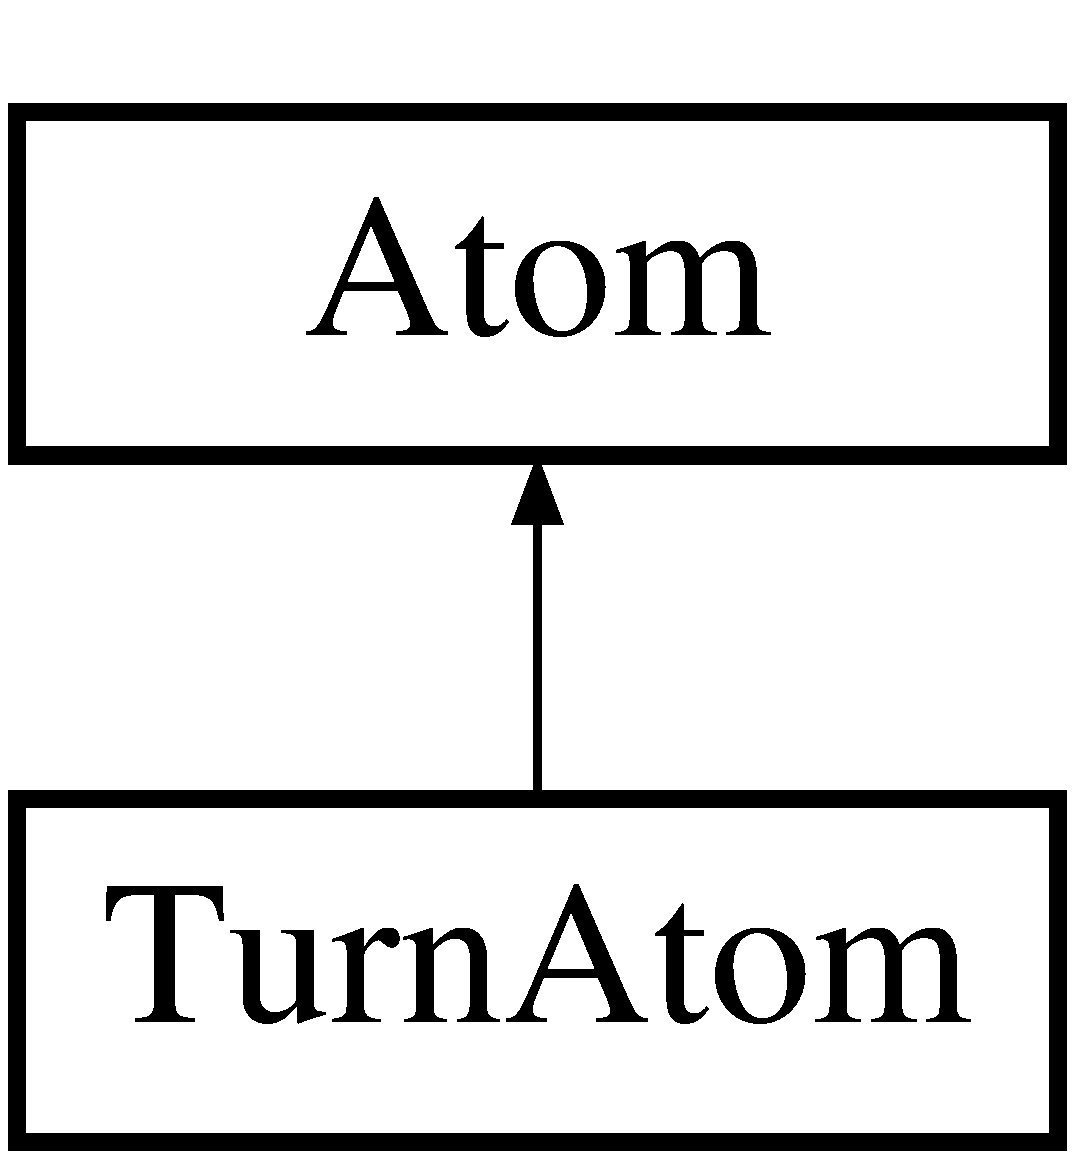
\includegraphics[height=2.000000cm]{class_turn_atom}
\end{center}
\end{figure}
\subsection*{Public Member Functions}
\begin{DoxyCompactItemize}
\item 
\hypertarget{class_turn_atom_adfc217157c5a658f963b1393f4903f5d}{{\bfseries Turn\-Atom} (float k\-P, float k\-I, float k\-D, C\-A\-N\-Jaguar $\ast$front\-Left, C\-A\-N\-Jaguar $\ast$rear\-Left, C\-A\-N\-Jaguar $\ast$front\-Right, C\-A\-N\-Jaguar $\ast$rear\-Right, Gyro $\ast$gyro, float angle)}\label{class_turn_atom_adfc217157c5a658f963b1393f4903f5d}

\item 
\hypertarget{class_turn_atom_ab8a0b59dd3d894aa1559f1a608a280e2}{void {\bfseries Execute} ()}\label{class_turn_atom_ab8a0b59dd3d894aa1559f1a608a280e2}

\end{DoxyCompactItemize}
\subsection*{Additional Inherited Members}


The documentation for this class was generated from the following files\-:\begin{DoxyCompactItemize}
\item 
Varun\-\_\-\-Atoms/Atom.\-h\item 
Varun\-\_\-\-Atoms/Atom.\-cpp\end{DoxyCompactItemize}

\hypertarget{class_wrist_atom}{\section{Wrist\-Atom Class Reference}
\label{class_wrist_atom}\index{Wrist\-Atom@{Wrist\-Atom}}
}
Inheritance diagram for Wrist\-Atom\-:\begin{figure}[H]
\begin{center}
\leavevmode
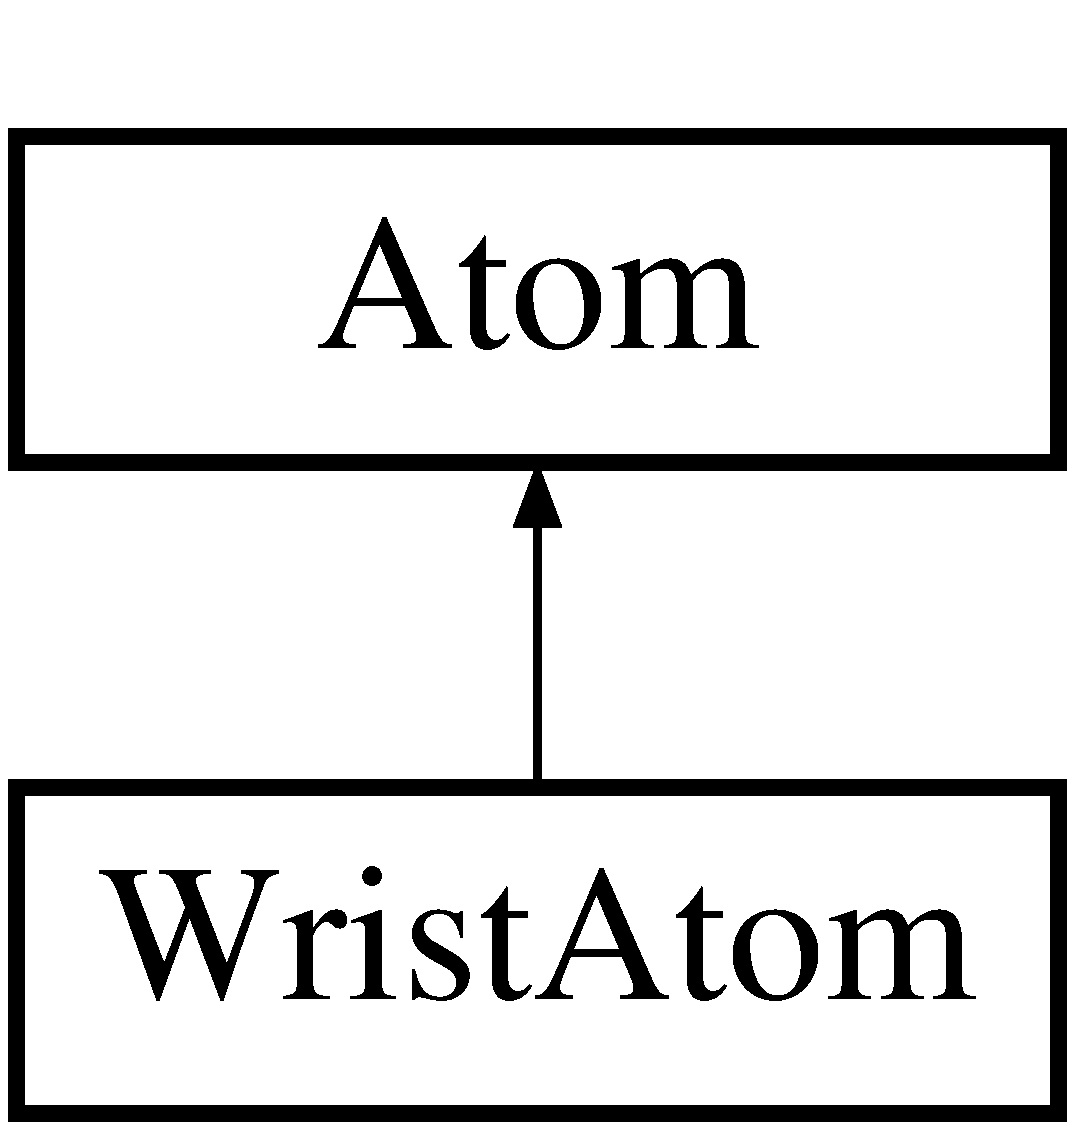
\includegraphics[height=2.000000cm]{class_wrist_atom}
\end{center}
\end{figure}
\subsection*{Public Member Functions}
\begin{DoxyCompactItemize}
\item 
\hypertarget{class_wrist_atom_a599f2334fe2ad70e3694b5838a304e1b}{{\bfseries Wrist\-Atom} (C\-A\-N\-Jaguar $\ast$front\-Left, C\-A\-N\-Jaguar $\ast$rear\-Left, C\-A\-N\-Jaguar $\ast$front\-Right, C\-A\-N\-Jaguar $\ast$rear\-Right)}\label{class_wrist_atom_a599f2334fe2ad70e3694b5838a304e1b}

\item 
\hypertarget{class_wrist_atom_a6d48f7678a4140dc893ad71c2462007b}{void {\bfseries Execute} ()}\label{class_wrist_atom_a6d48f7678a4140dc893ad71c2462007b}

\end{DoxyCompactItemize}
\subsection*{Additional Inherited Members}


The documentation for this class was generated from the following files\-:\begin{DoxyCompactItemize}
\item 
Varun\-\_\-\-Atoms/Atom.\-h\item 
Varun\-\_\-\-Atoms/Atom.\-cpp\end{DoxyCompactItemize}

\printindex
\end{document}
